\documentclass[11pt,a4paper]{article}
\usepackage[margin=1in]{geometry}
\usepackage{graphicx}
\usepackage{booktabs}
\usepackage{caption}
\usepackage{subcaption}
\usepackage{float}
\usepackage{xcolor}
\usepackage{hyperref}
\usepackage[skip=4pt]{parskip}
\hypersetup{colorlinks=true, linkcolor=blue!60!black, urlcolor=blue!60!black}
\graphicspath{{figures/}{figures/per_plant/}}

\title{EmbodiedMAE-4M: A Multi-modal Masked Autoencoder for Synthetic Sorghum \\[2pt] \large run~v3 -- 2400-epoch completion report}
\author{Alloy Das \\ Iowa State University \\ \texttt{alloydas@iastate.edu}}
\date{\today}

\begin{document}
\maketitle

\begin{abstract}
EmbodiedMAE-4M is a four-modality masked autoencoder pre-trained on synthetic sorghum plants rendered from a procedural generator. Each sample bundles an aligned RGB image, a depth map, a point cloud, and the underlying procedural parameters (plant + per-leaf), and a single transformer encoder is asked to reconstruct all four after Dirichlet-allocated token masking.
This report covers run~v3, which trained for 2400 epochs on the synthetic dataset at \texttt{mask\_ratio} $= 0.15$ and reached its best held-out validation loss of 0.0204 at epoch~2280 (parameter accuracy at $|\Delta| < 0.05$ of 100.00\%). We include the architecture diagram, full training curves, per-modality metrics, and a 15-plant reconstruction gallery.
\end{abstract}

\section{Architecture}
A shared ViT-base encoder ingests visible tokens from all four modalities and a per-modality decoder reconstructs the masked tokens. Modality embeddings: RGB/depth via patch embedding ($196$ tokens at $224{\times}224$, patch~$16$); point cloud via FPS centres ($196$ tokens) + kNN grouping ($k{=}32$) feeding a PointNet-style MLP; spline parameters via char + positional embeddings mean-pooled per token ($1$ plant token $+$ up to $24$ leaf tokens). A single Dirichlet draw per training step decides the per-modality fraction of visible tokens; the 4M variant also enforces \texttt{min\_mask\_ratio}~$=0.25$ per modality.

\begin{figure}[H]
\centering
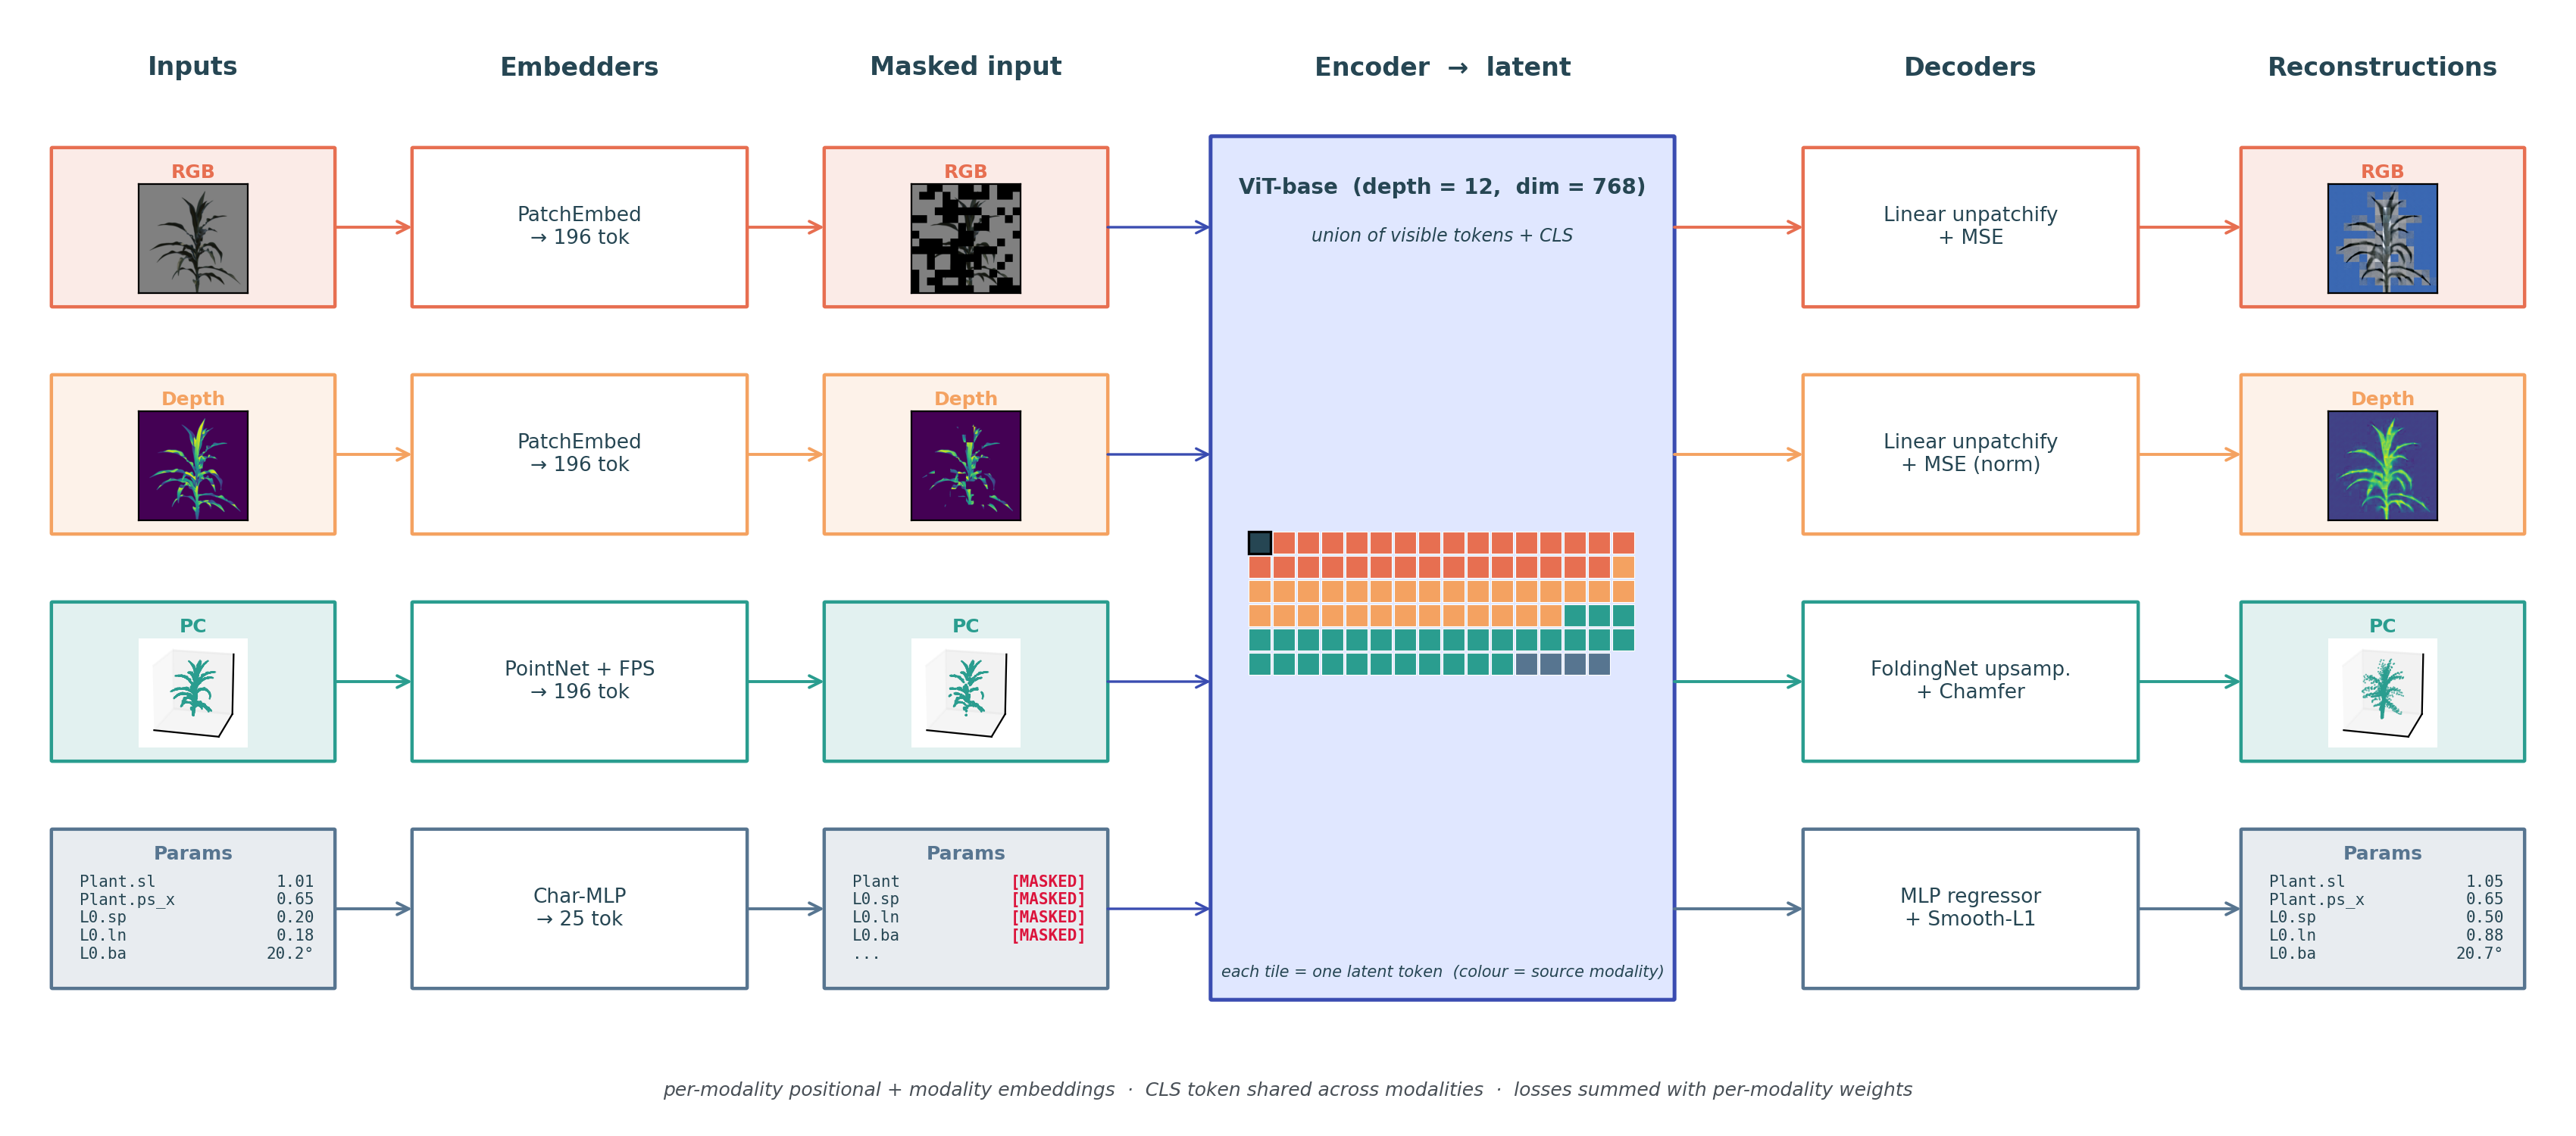
\includegraphics[width=\linewidth]{arch_diagram.png}
\caption{EmbodiedMAE-4M architecture. RGB, depth, point cloud, and spline/parameter tokens are embedded, masked under a Dirichlet allocation, fed through a shared encoder, and reconstructed by four modality-specific decoder heads.}
\label{fig:arch}
\end{figure}

\section{Training setup}
\begin{table}[H]
\centering
\caption{Run~v3 training configuration.}
\label{tab:setup}
\begin{tabular}{ll}
\toprule
Key & Value \\
\midrule
Dataset & synthetic sorghum (10\,000 train / 100 val) \\
Image size & $224 \times 224$ (patch $16$) \\
Point cloud & $8\,196$ points, unit-sphere normalised, FPS centres $=196$, kNN $k=32$ \\
Max leaves per plant & $24$ (padded) \\
Model size & base ($\sim$114\,M params, $d=768$, depth $12$ enc / $8$ dec) \\
Mask ratio (train) & $0.15$ (Dirichlet over modalities, min $0.25$ per modality) \\
Loss weights & RGB $1$, Depth $1$, PC $10$ (Chamfer), Params $5$ (Smooth-L1) \\
Optimizer & AdamW, weight decay $0.05$ \\
LR schedule & $1.5\!\times\!10^{-4}$ peak, $10$-epoch linear warmup, cosine decay \\
Batch / GPU & $16$ on H200 (resumed run); effective batch $16$ \\
Epochs & $1$ -- $2400$ (completed) \\
Validation interval & every $20$ epochs \\
\bottomrule
\end{tabular}
\end{table}

\section{Training dynamics}
Figure~\ref{fig:curves} shows per-modality train and validation losses on a log scale across all 2400 epochs, plus the parameter accuracy at $|\Delta|<0.05$ and the cosine LR schedule. The dashed vertical marks the best-validation epoch (\textbf{2280}); the total loss is the sum of the weighted modality terms, so the small PC and text terms appear close to the floor on the log axis but are reported separately in Table~\ref{tab:metrics}.

\begin{figure}[H]
\centering
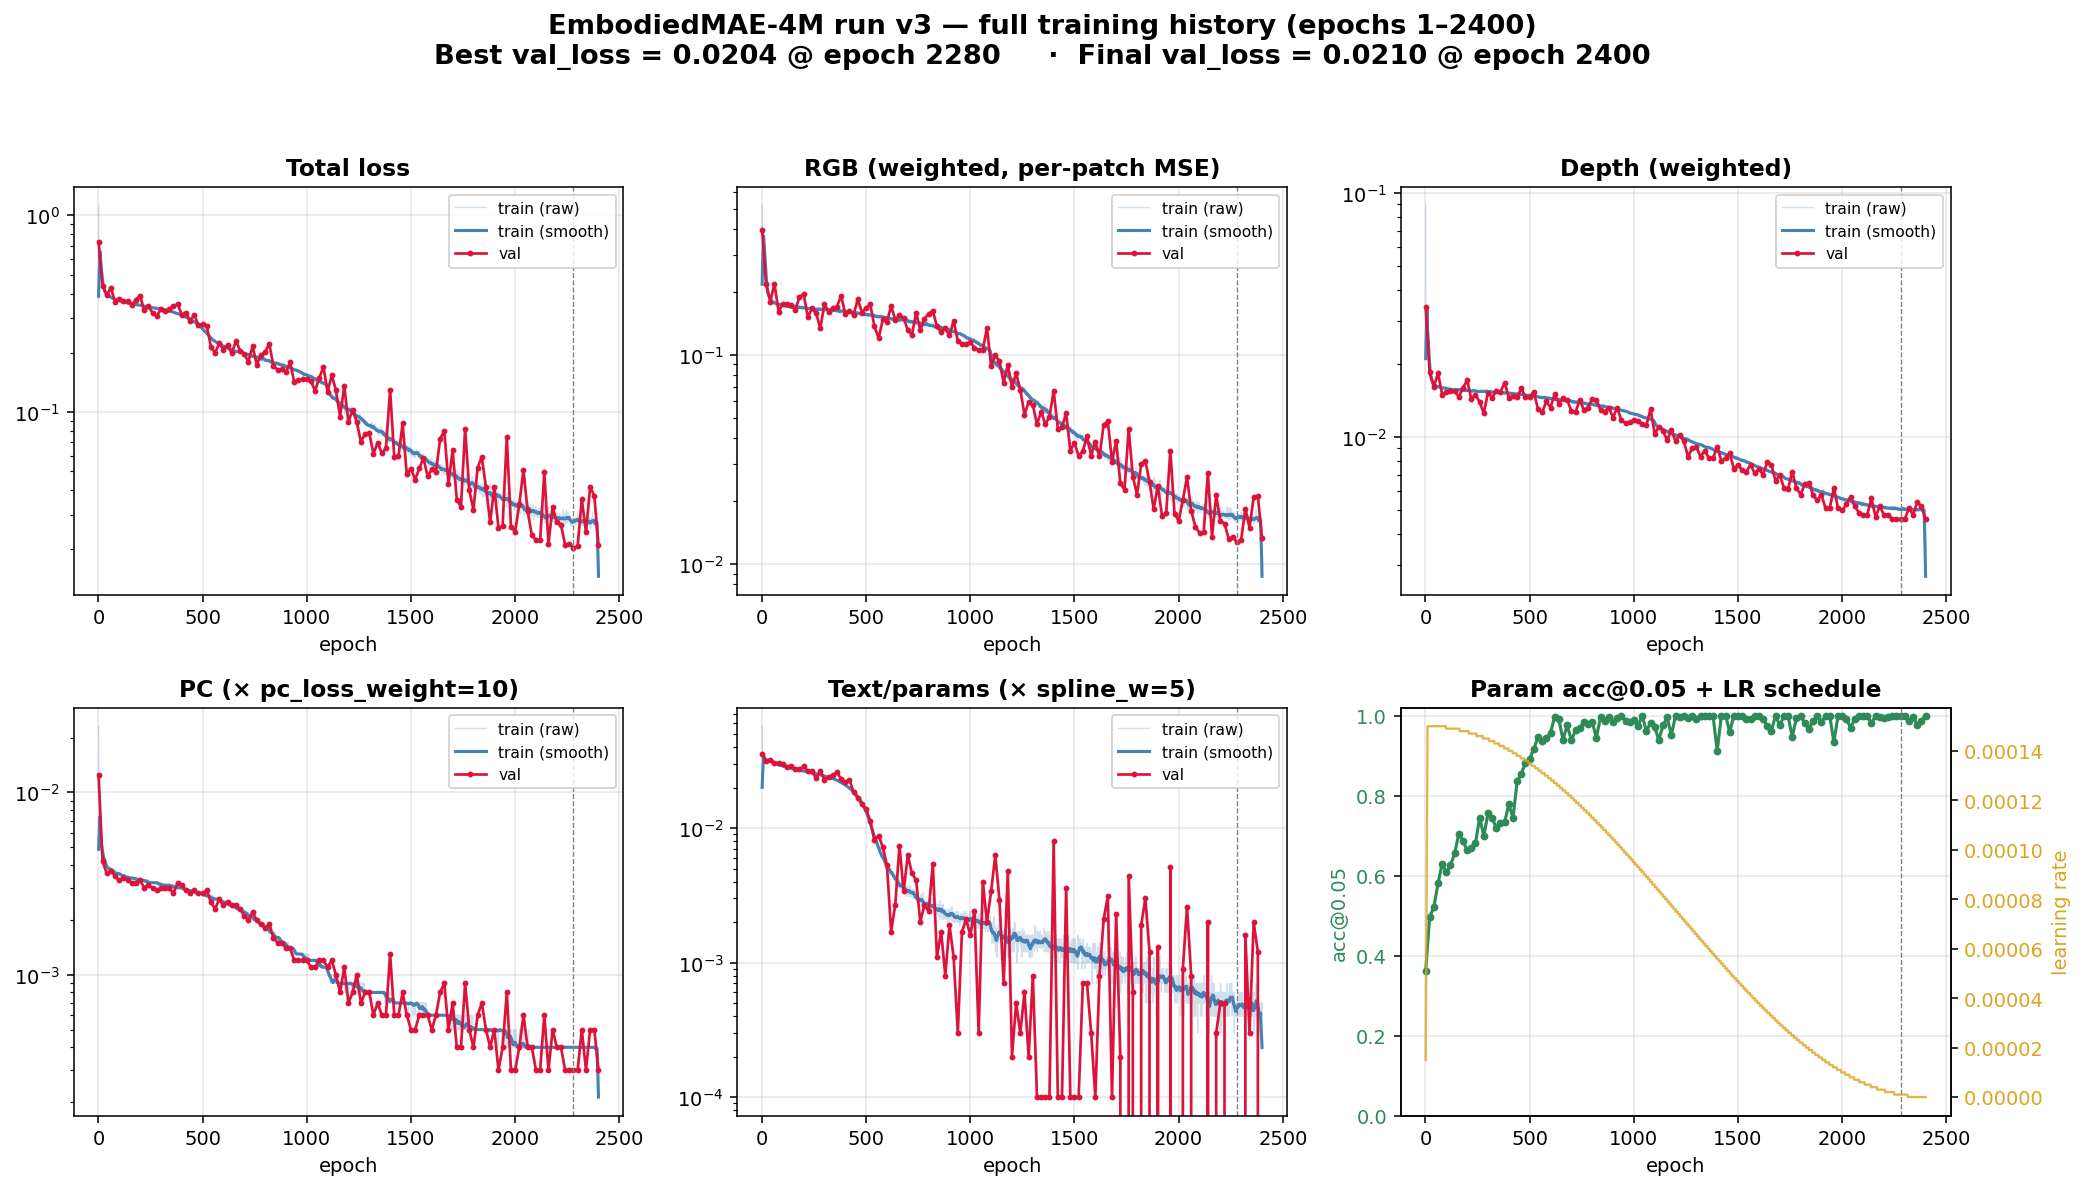
\includegraphics[width=\linewidth]{loss_curves_2400.png}
\caption{Per-modality train (blue, raw and 15-epoch smoothed) and validation (red) losses across the full 2400-epoch run, plus parameter accuracy@$0.05$ and LR schedule.}
\label{fig:curves}
\end{figure}

\section{Validation metrics}
\begin{table}[H]
\centering
\caption{Validation metrics at the best epoch (lowest \texttt{val\_loss}) and at the final epoch. Weighted columns use the training loss weights; the lower block reports raw modality metrics. \texttt{param\_acc05} counts predictions within $|\Delta| < 0.05$ in normalised parameter space.}
\label{tab:metrics}
\begin{tabular}{lrr}
\toprule
Metric & Best (ep~2280) & Final (ep~2400) \\
\midrule
val\_loss (weighted total) & 0.0204 & 0.0210 \\
val\_rgb (per-patch MSE) & 0.0127 & 0.0133 \\
val\_depth (per-patch MSE) & 0.0046 & 0.0046 \\
val\_pc ($\times$ 10) & 0.0003 & 0.0003 \\
val\_text ($\times$ 5) & 0.0000 & 0.0000 \\
\midrule
RGB MSE (unweighted) & 0.6976 & 0.6977 \\
Depth MSE (on min-max target) & 0.0071 & 0.0070 \\
PC Chamfer (bidirectional) & 0.000308 & 0.000299 \\
Param MSE (Smooth-L1 surrogate) & 0.0168 & 0.0165 \\
Param MAE (all leaves) & 0.0568 & 0.0546 \\
Param MAE (masked tokens) & 0.001025 & 0.001052 \\
Param acc@$0.05$ & 100.00\% & 100.00\% \\
\bottomrule
\end{tabular}
\end{table}

\section{Held-out evaluation on the 15-plant gallery}
For the reconstruction gallery (Figure~\ref{fig:gallery}) we ran the checkpoint at epoch \textbf{2400} on 15 validation plants at a higher \texttt{mask\_ratio} of 0.40 so the masking pattern is visible. The aggregate metrics (Table~\ref{tab:eval}) confirm the reconstruction quality holds up under more aggressive masking.

\begin{table}[H]
\centering
\caption{Aggregate metrics over the 15-plant evaluation dump at \texttt{mask\_ratio} = 0.40.}
\label{tab:eval}
\begin{tabular}{lr}
\toprule
Metric & Value \\
\midrule
RGB MSE & 0.6878 \\
Depth MSE & 0.0077 \\
PC Chamfer (bidirectional) & 0.000500 \\
PC EMD (skipped) & 0.0000 \\
Param MAE (all) & 0.0518 \\
Param MAE (masked tokens) & 0.001495 \\
Number of plants & 15 \\
\bottomrule
\end{tabular}
\end{table}

\begin{figure}[H]
\centering
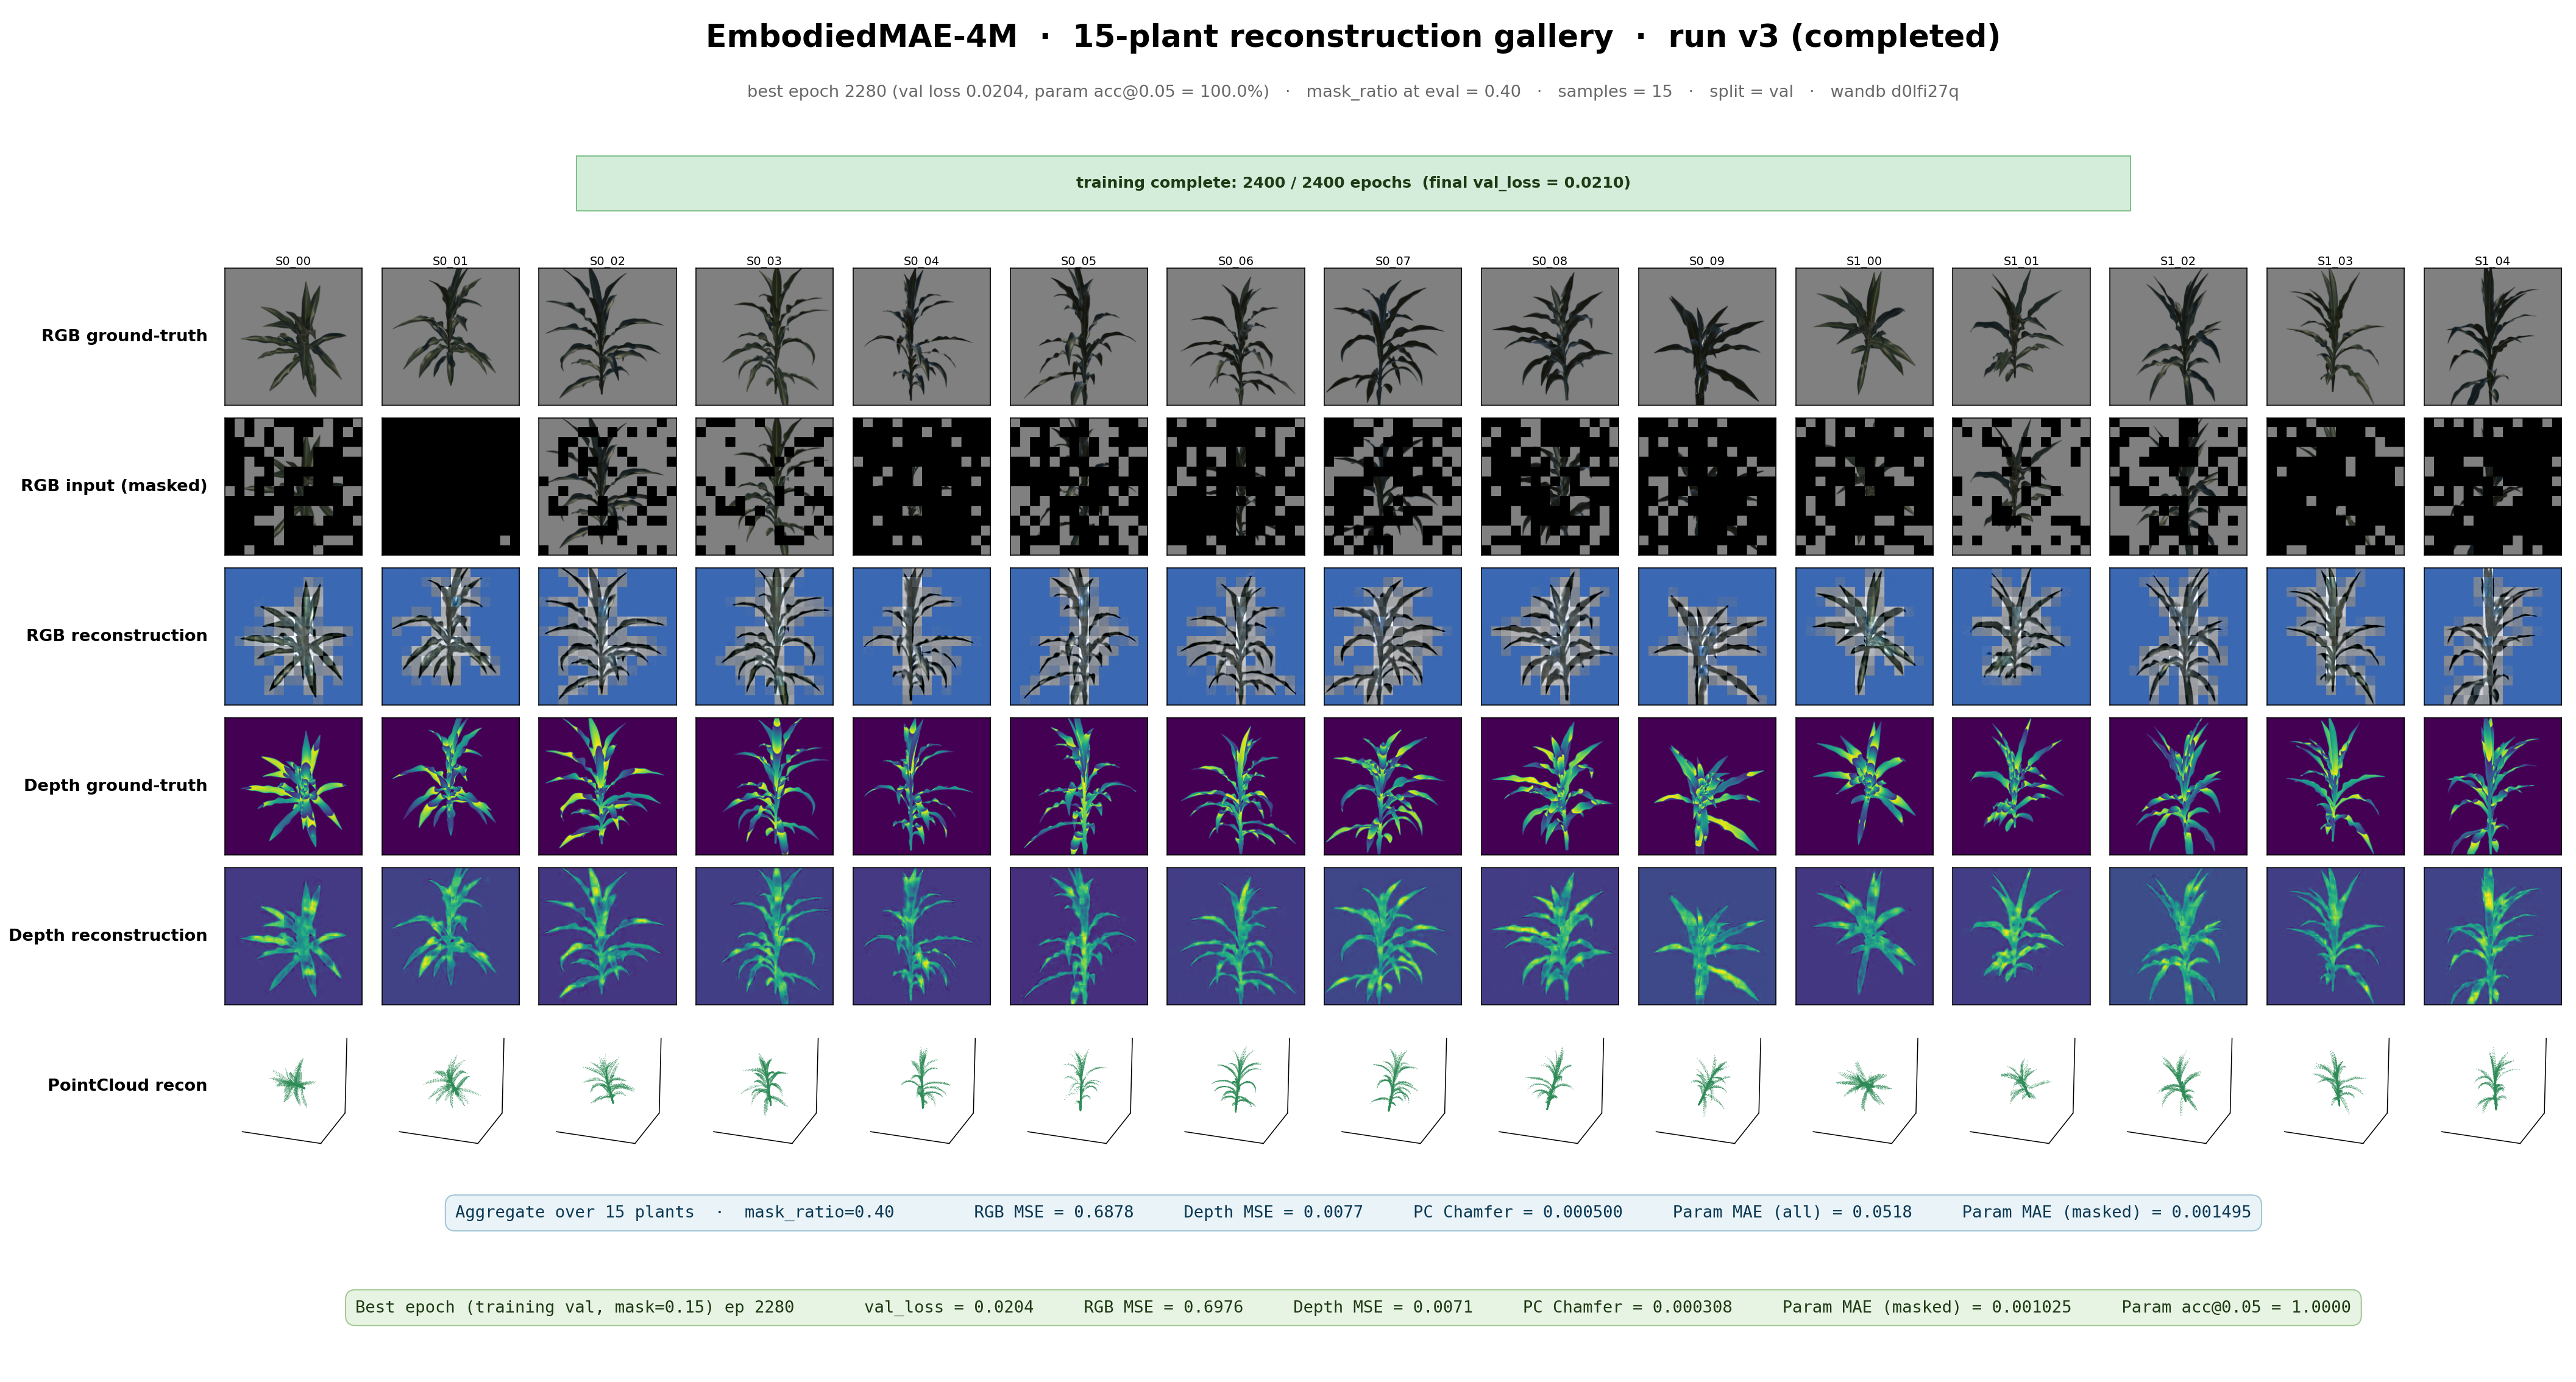
\includegraphics[width=\linewidth]{slide_figure_v3_2400.png}
\caption{15-plant reconstruction gallery at epoch~2400. Rows top-to-bottom: RGB ground truth, masked RGB input, RGB reconstruction, depth ground truth, depth reconstruction, point-cloud reconstruction (3D scatter). Each column is one validation plant.}
\label{fig:gallery}
\end{figure}
\clearpage

\section{Per-plant reconstruction figures}
Each figure below corresponds to one validation plant. From left to right: masked input, model reconstruction, ground truth. Modality rows: RGB, depth, point cloud, spline / procedural parameters. The right-hand panel lists every plant- and leaf-level parameter with the target, model prediction, and absolute difference; entries highlighted in red were masked at eval time.

\begin{figure}[H]
\centering
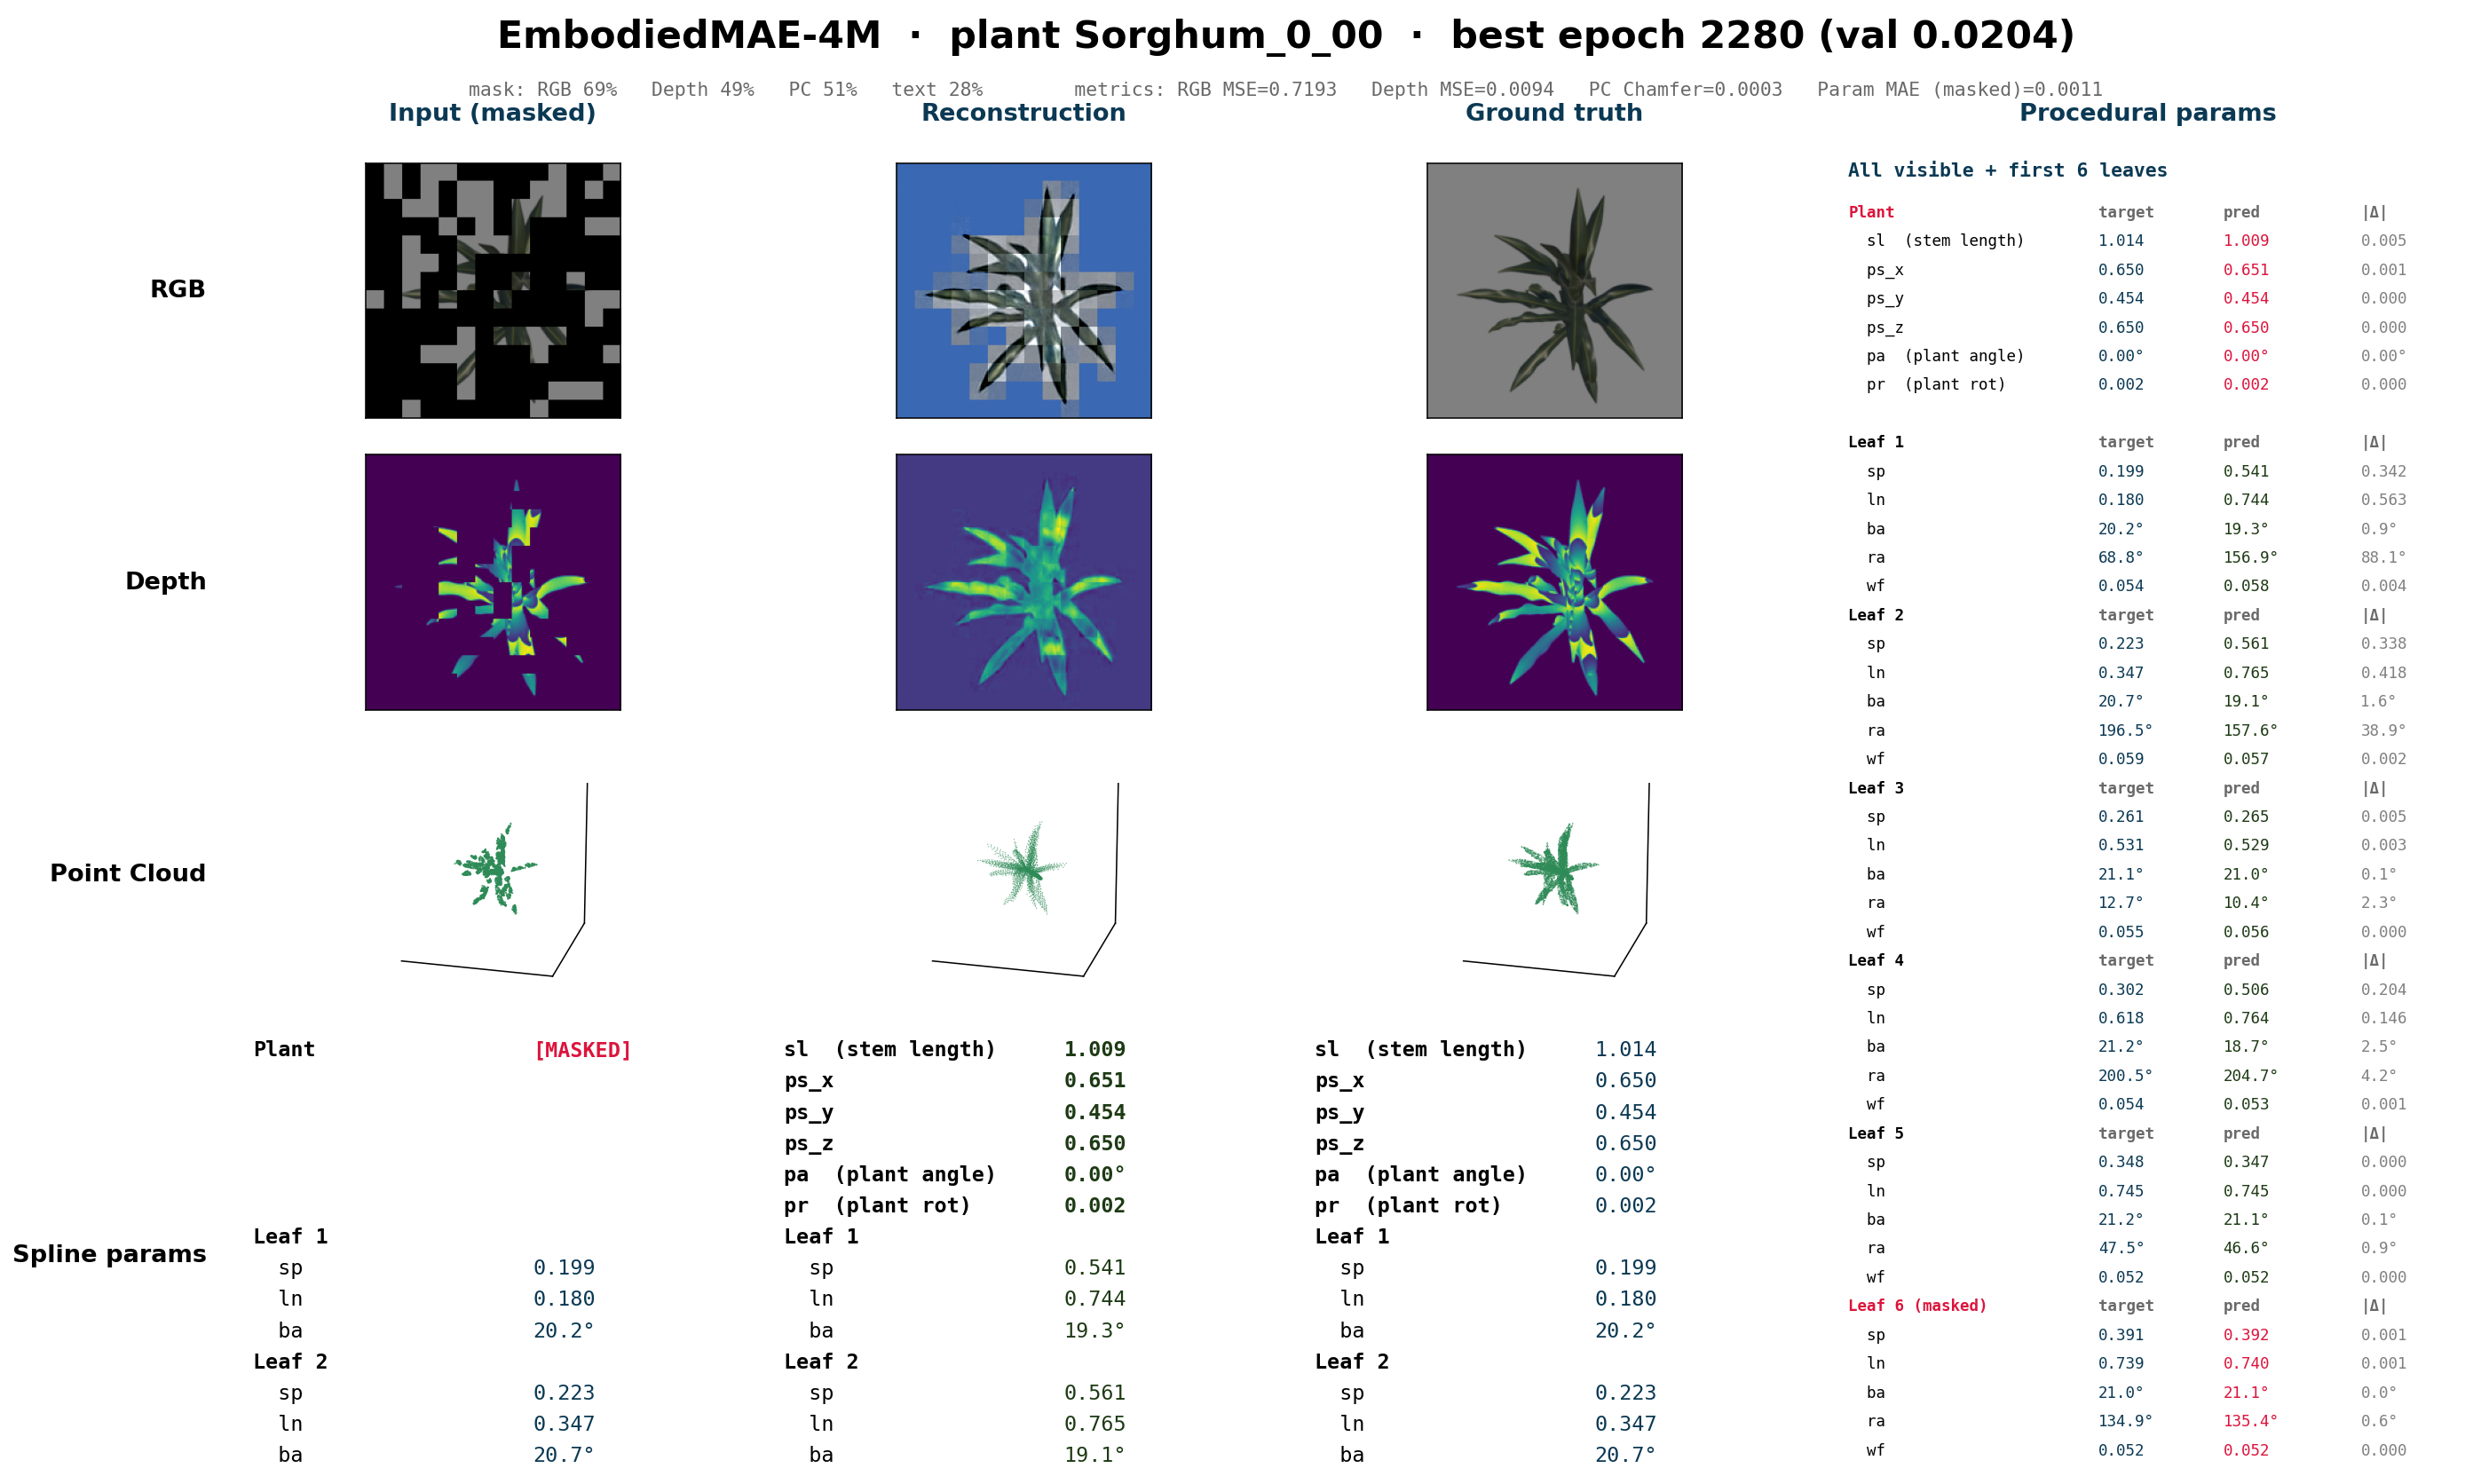
\includegraphics[width=\linewidth]{per_plant/Sorghum_0_00.png}
\caption{Plant Sorghum\_0\_00 -- epoch 2400 reconstruction.}
\label{fig:plant:Sorghum_0_00}
\end{figure}
\clearpage

\begin{figure}[H]
\centering
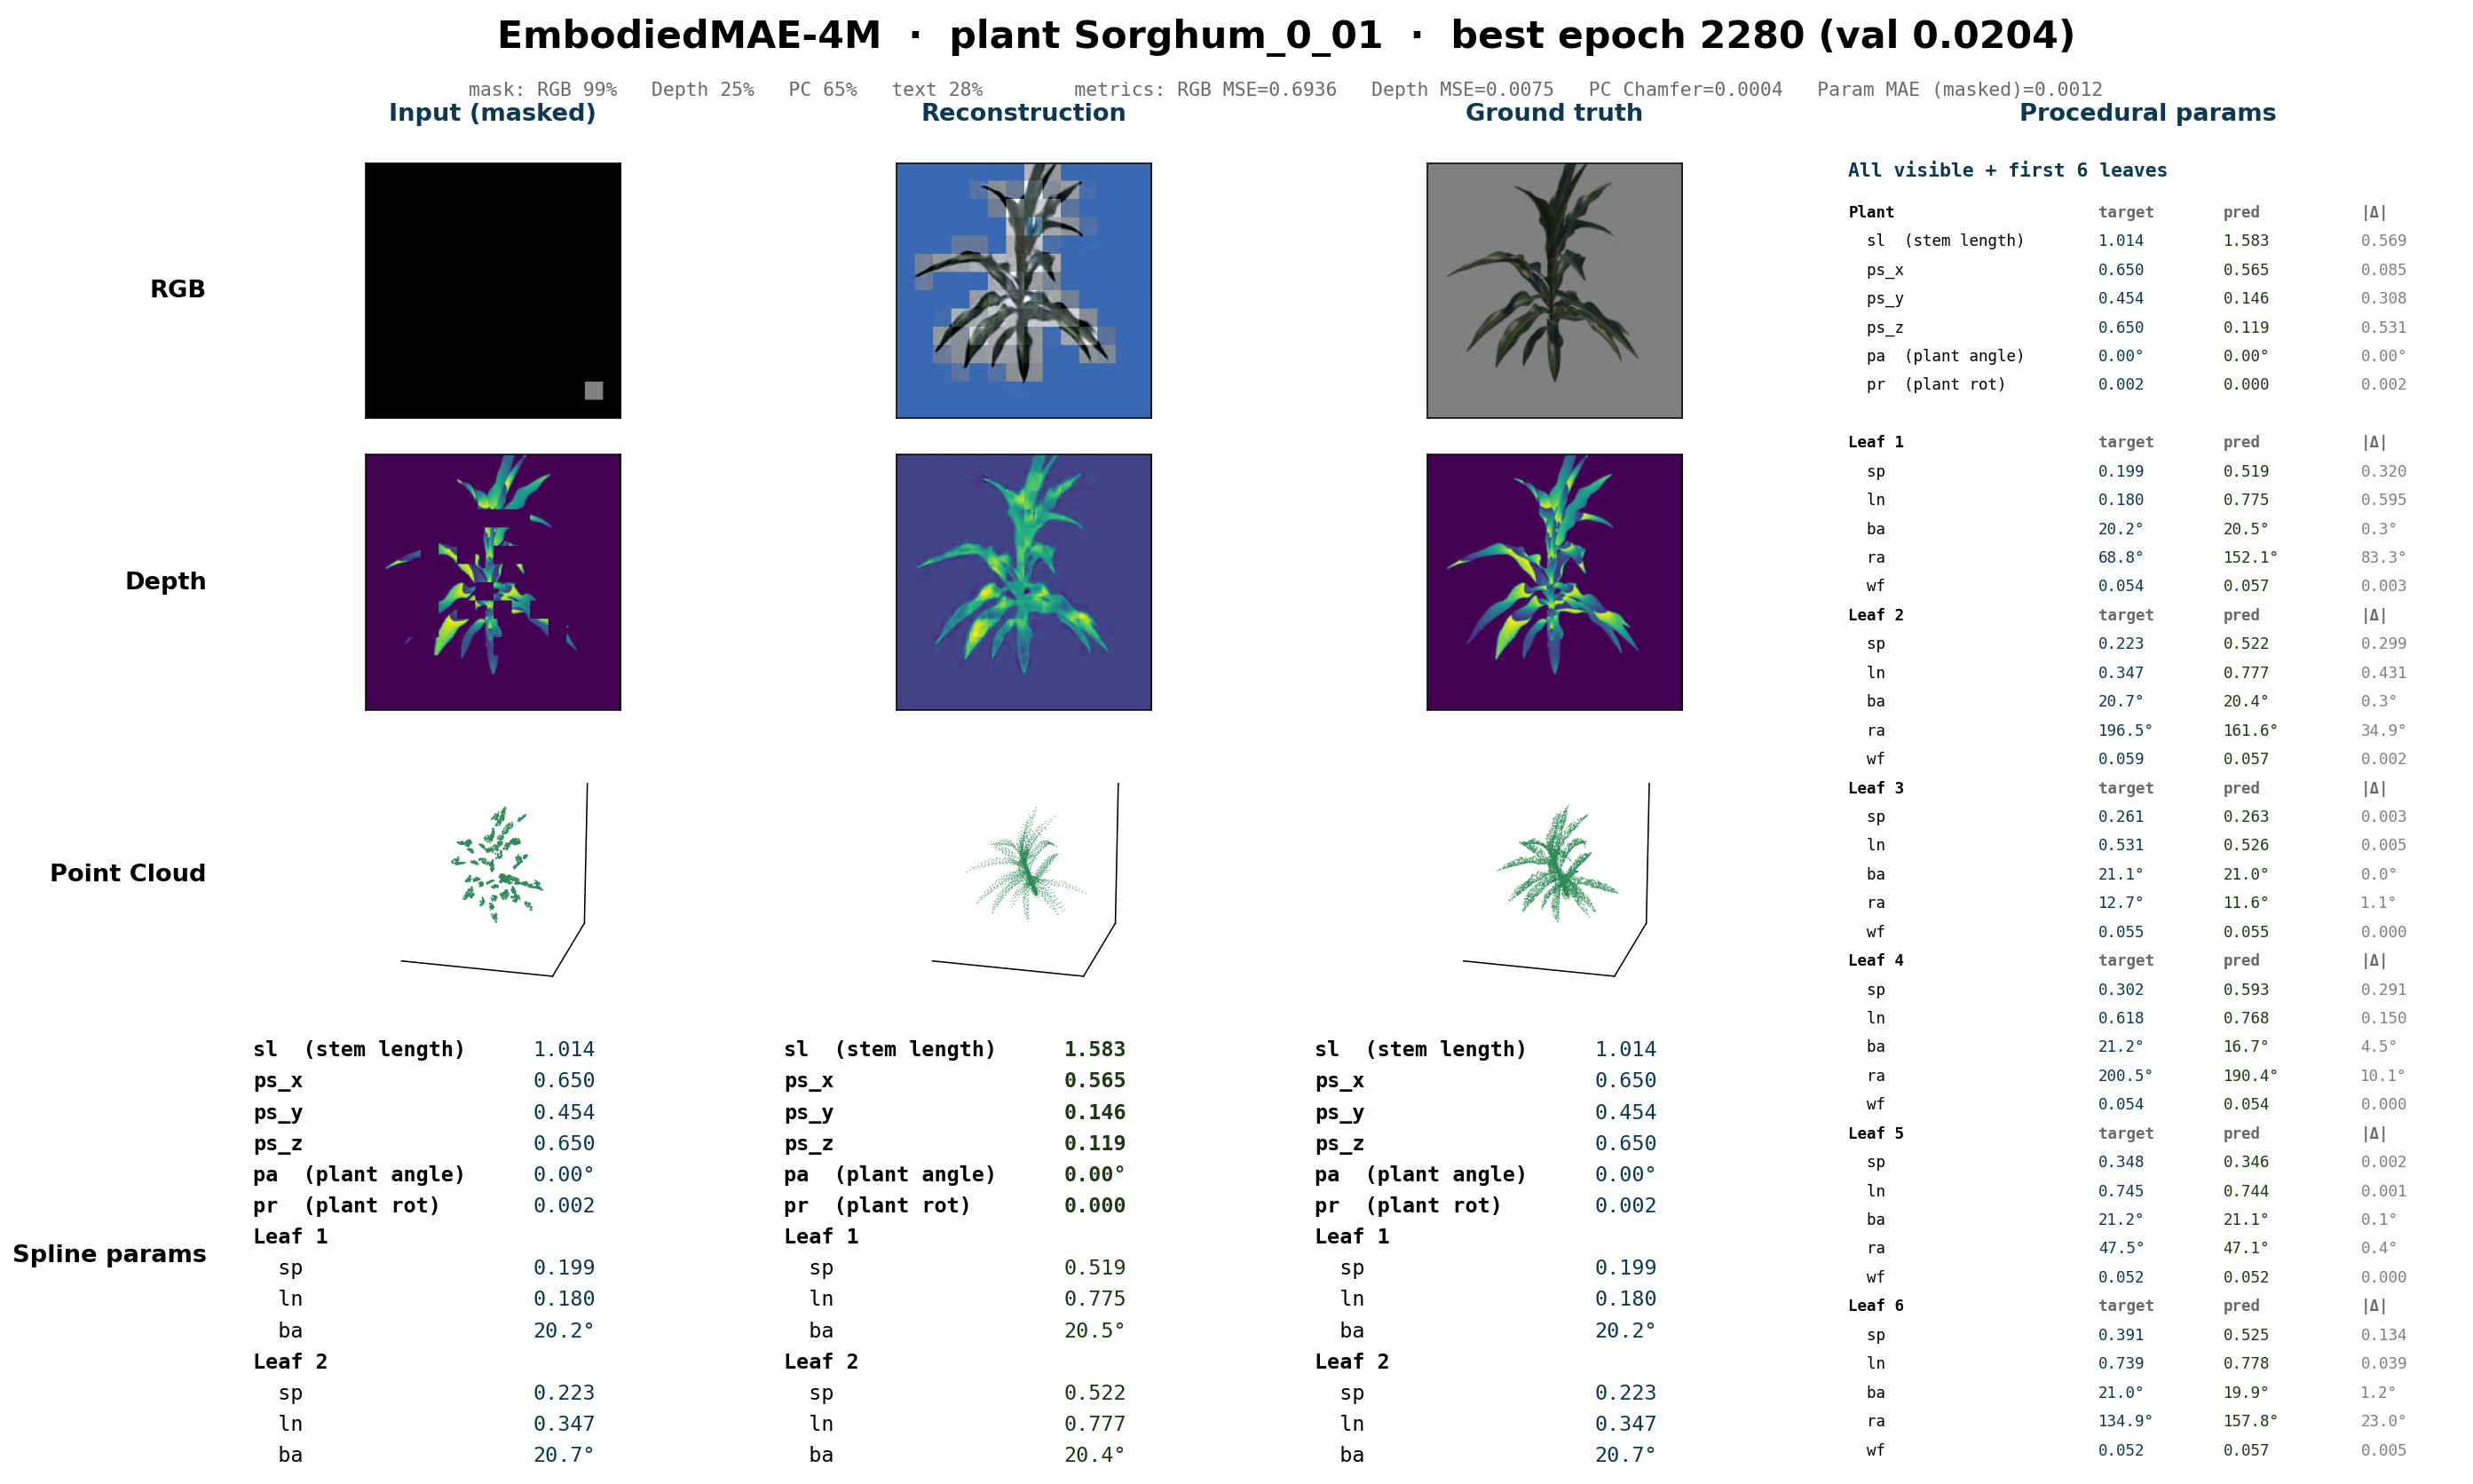
\includegraphics[width=\linewidth]{per_plant/Sorghum_0_01.png}
\caption{Plant Sorghum\_0\_01 -- epoch 2400 reconstruction.}
\label{fig:plant:Sorghum_0_01}
\end{figure}
\clearpage

\begin{figure}[H]
\centering
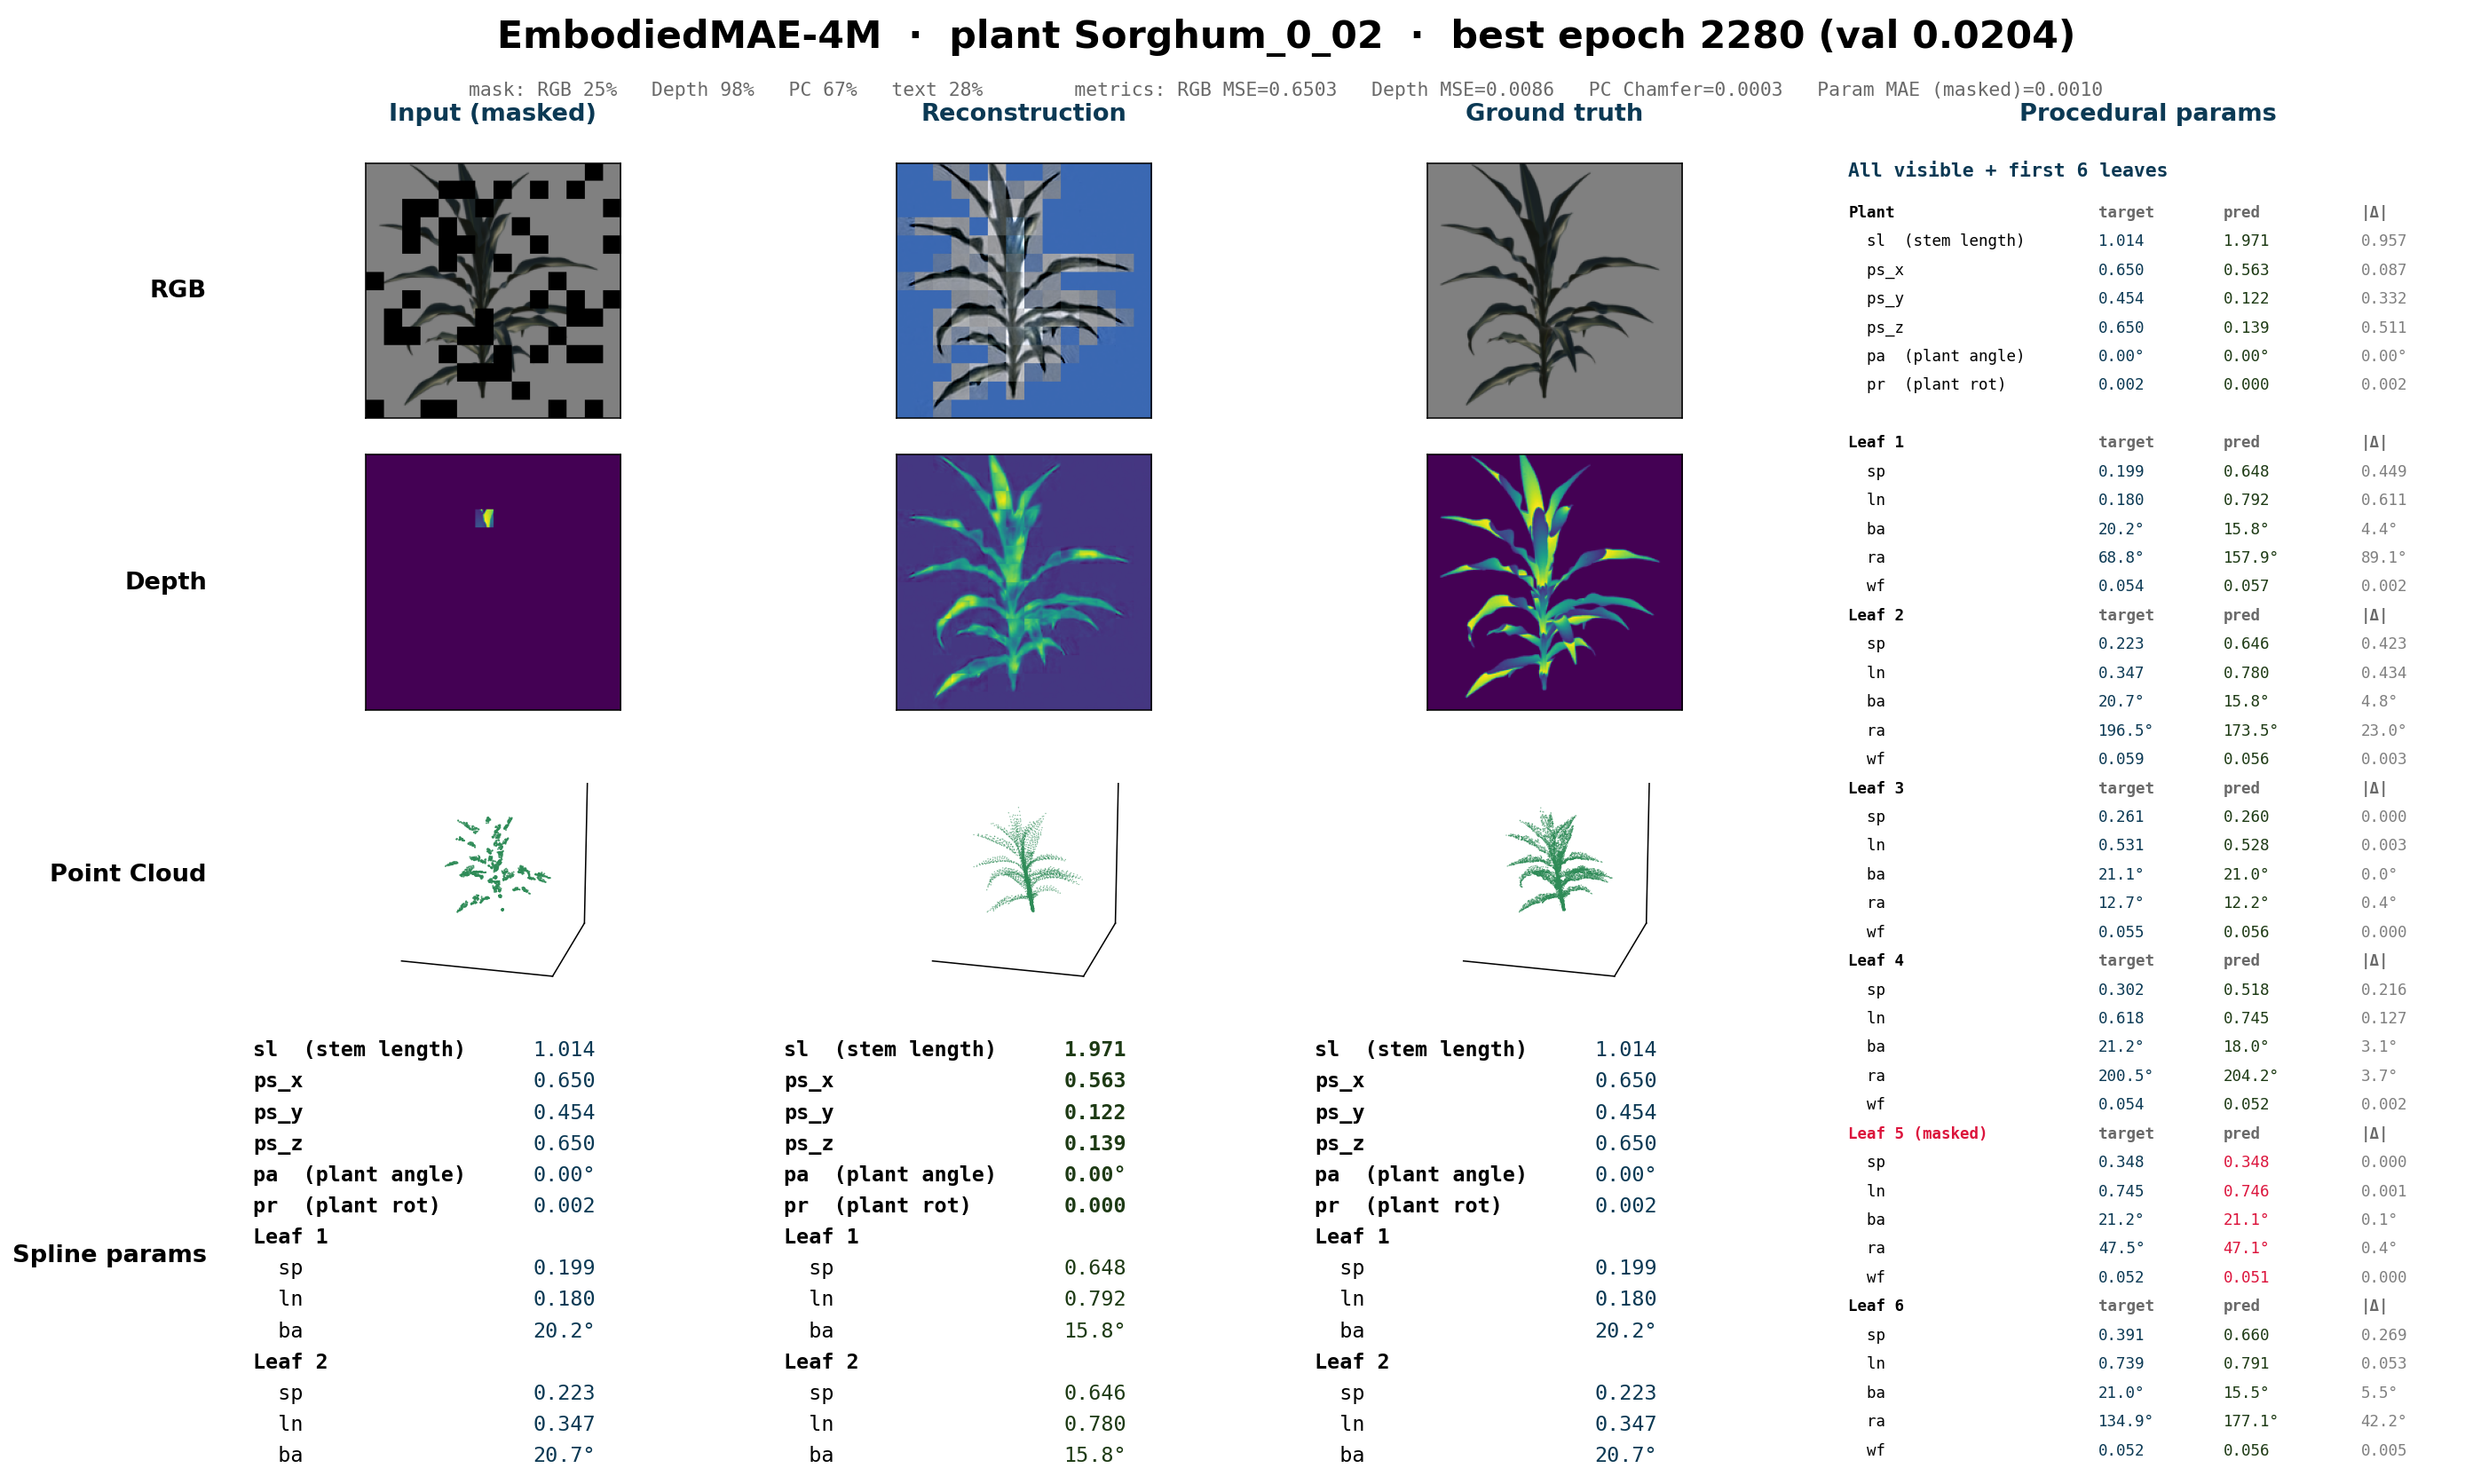
\includegraphics[width=\linewidth]{per_plant/Sorghum_0_02.png}
\caption{Plant Sorghum\_0\_02 -- epoch 2400 reconstruction.}
\label{fig:plant:Sorghum_0_02}
\end{figure}
\clearpage

\begin{figure}[H]
\centering
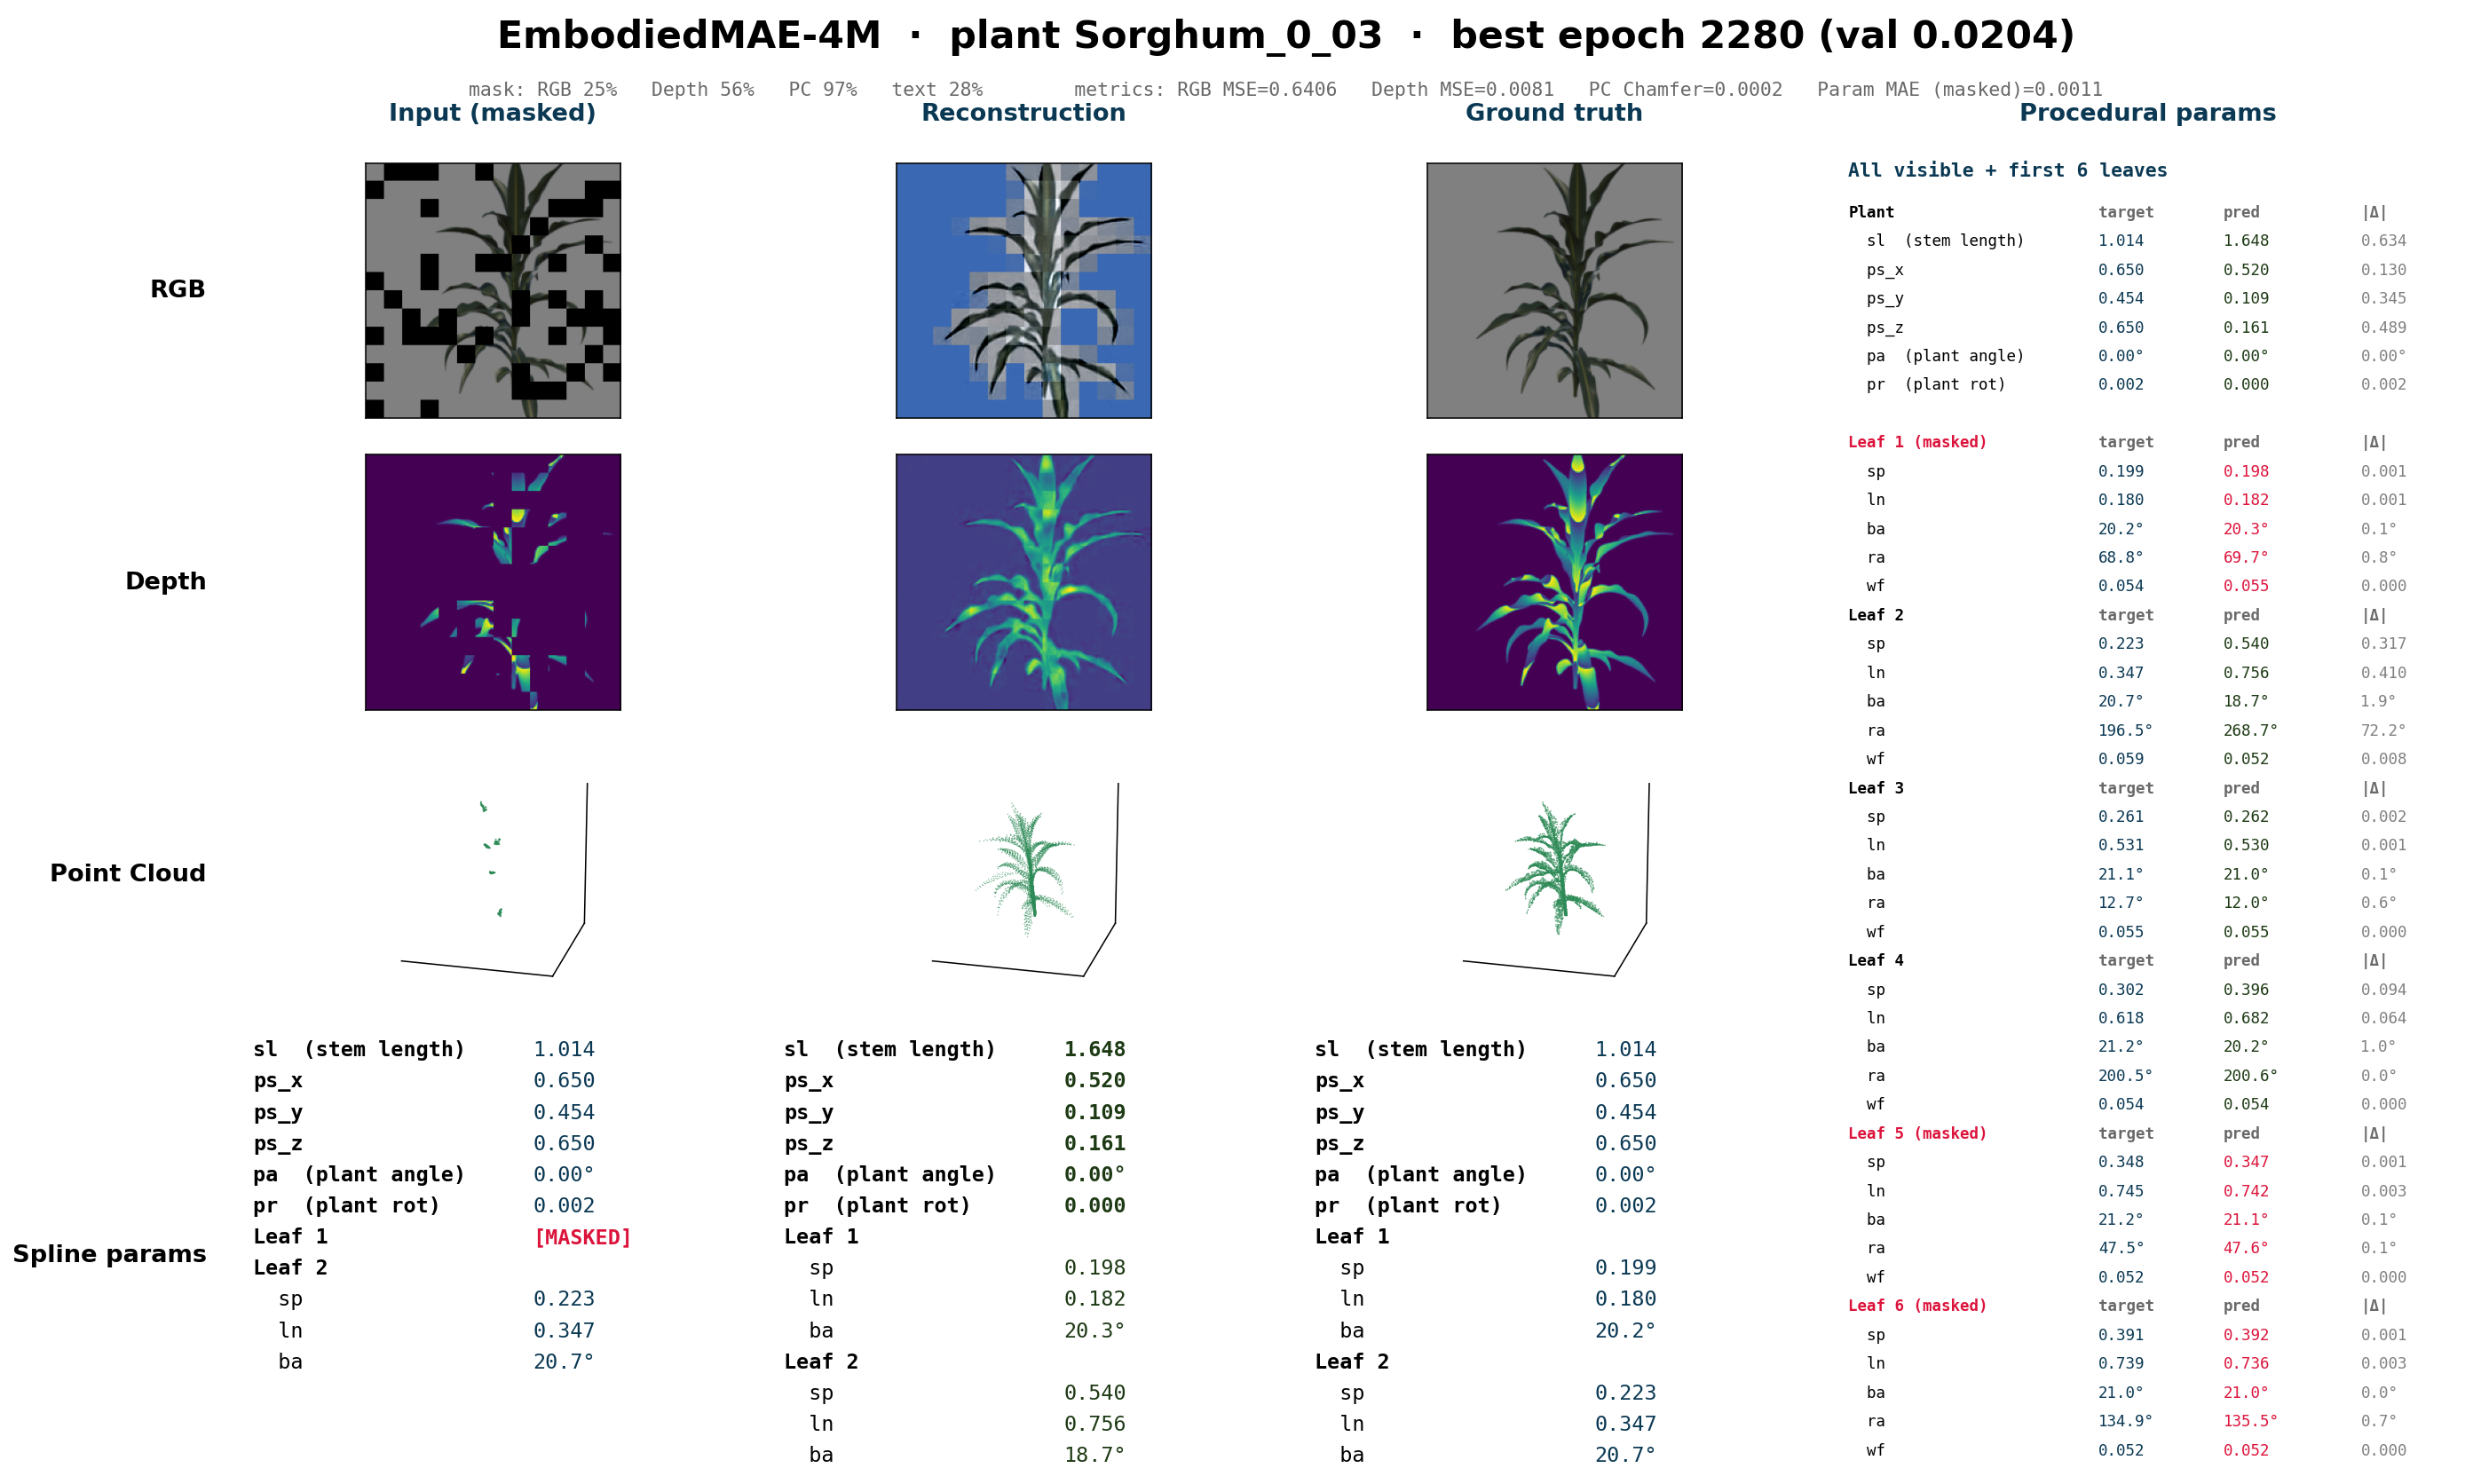
\includegraphics[width=\linewidth]{per_plant/Sorghum_0_03.png}
\caption{Plant Sorghum\_0\_03 -- epoch 2400 reconstruction.}
\label{fig:plant:Sorghum_0_03}
\end{figure}
\clearpage

\begin{figure}[H]
\centering
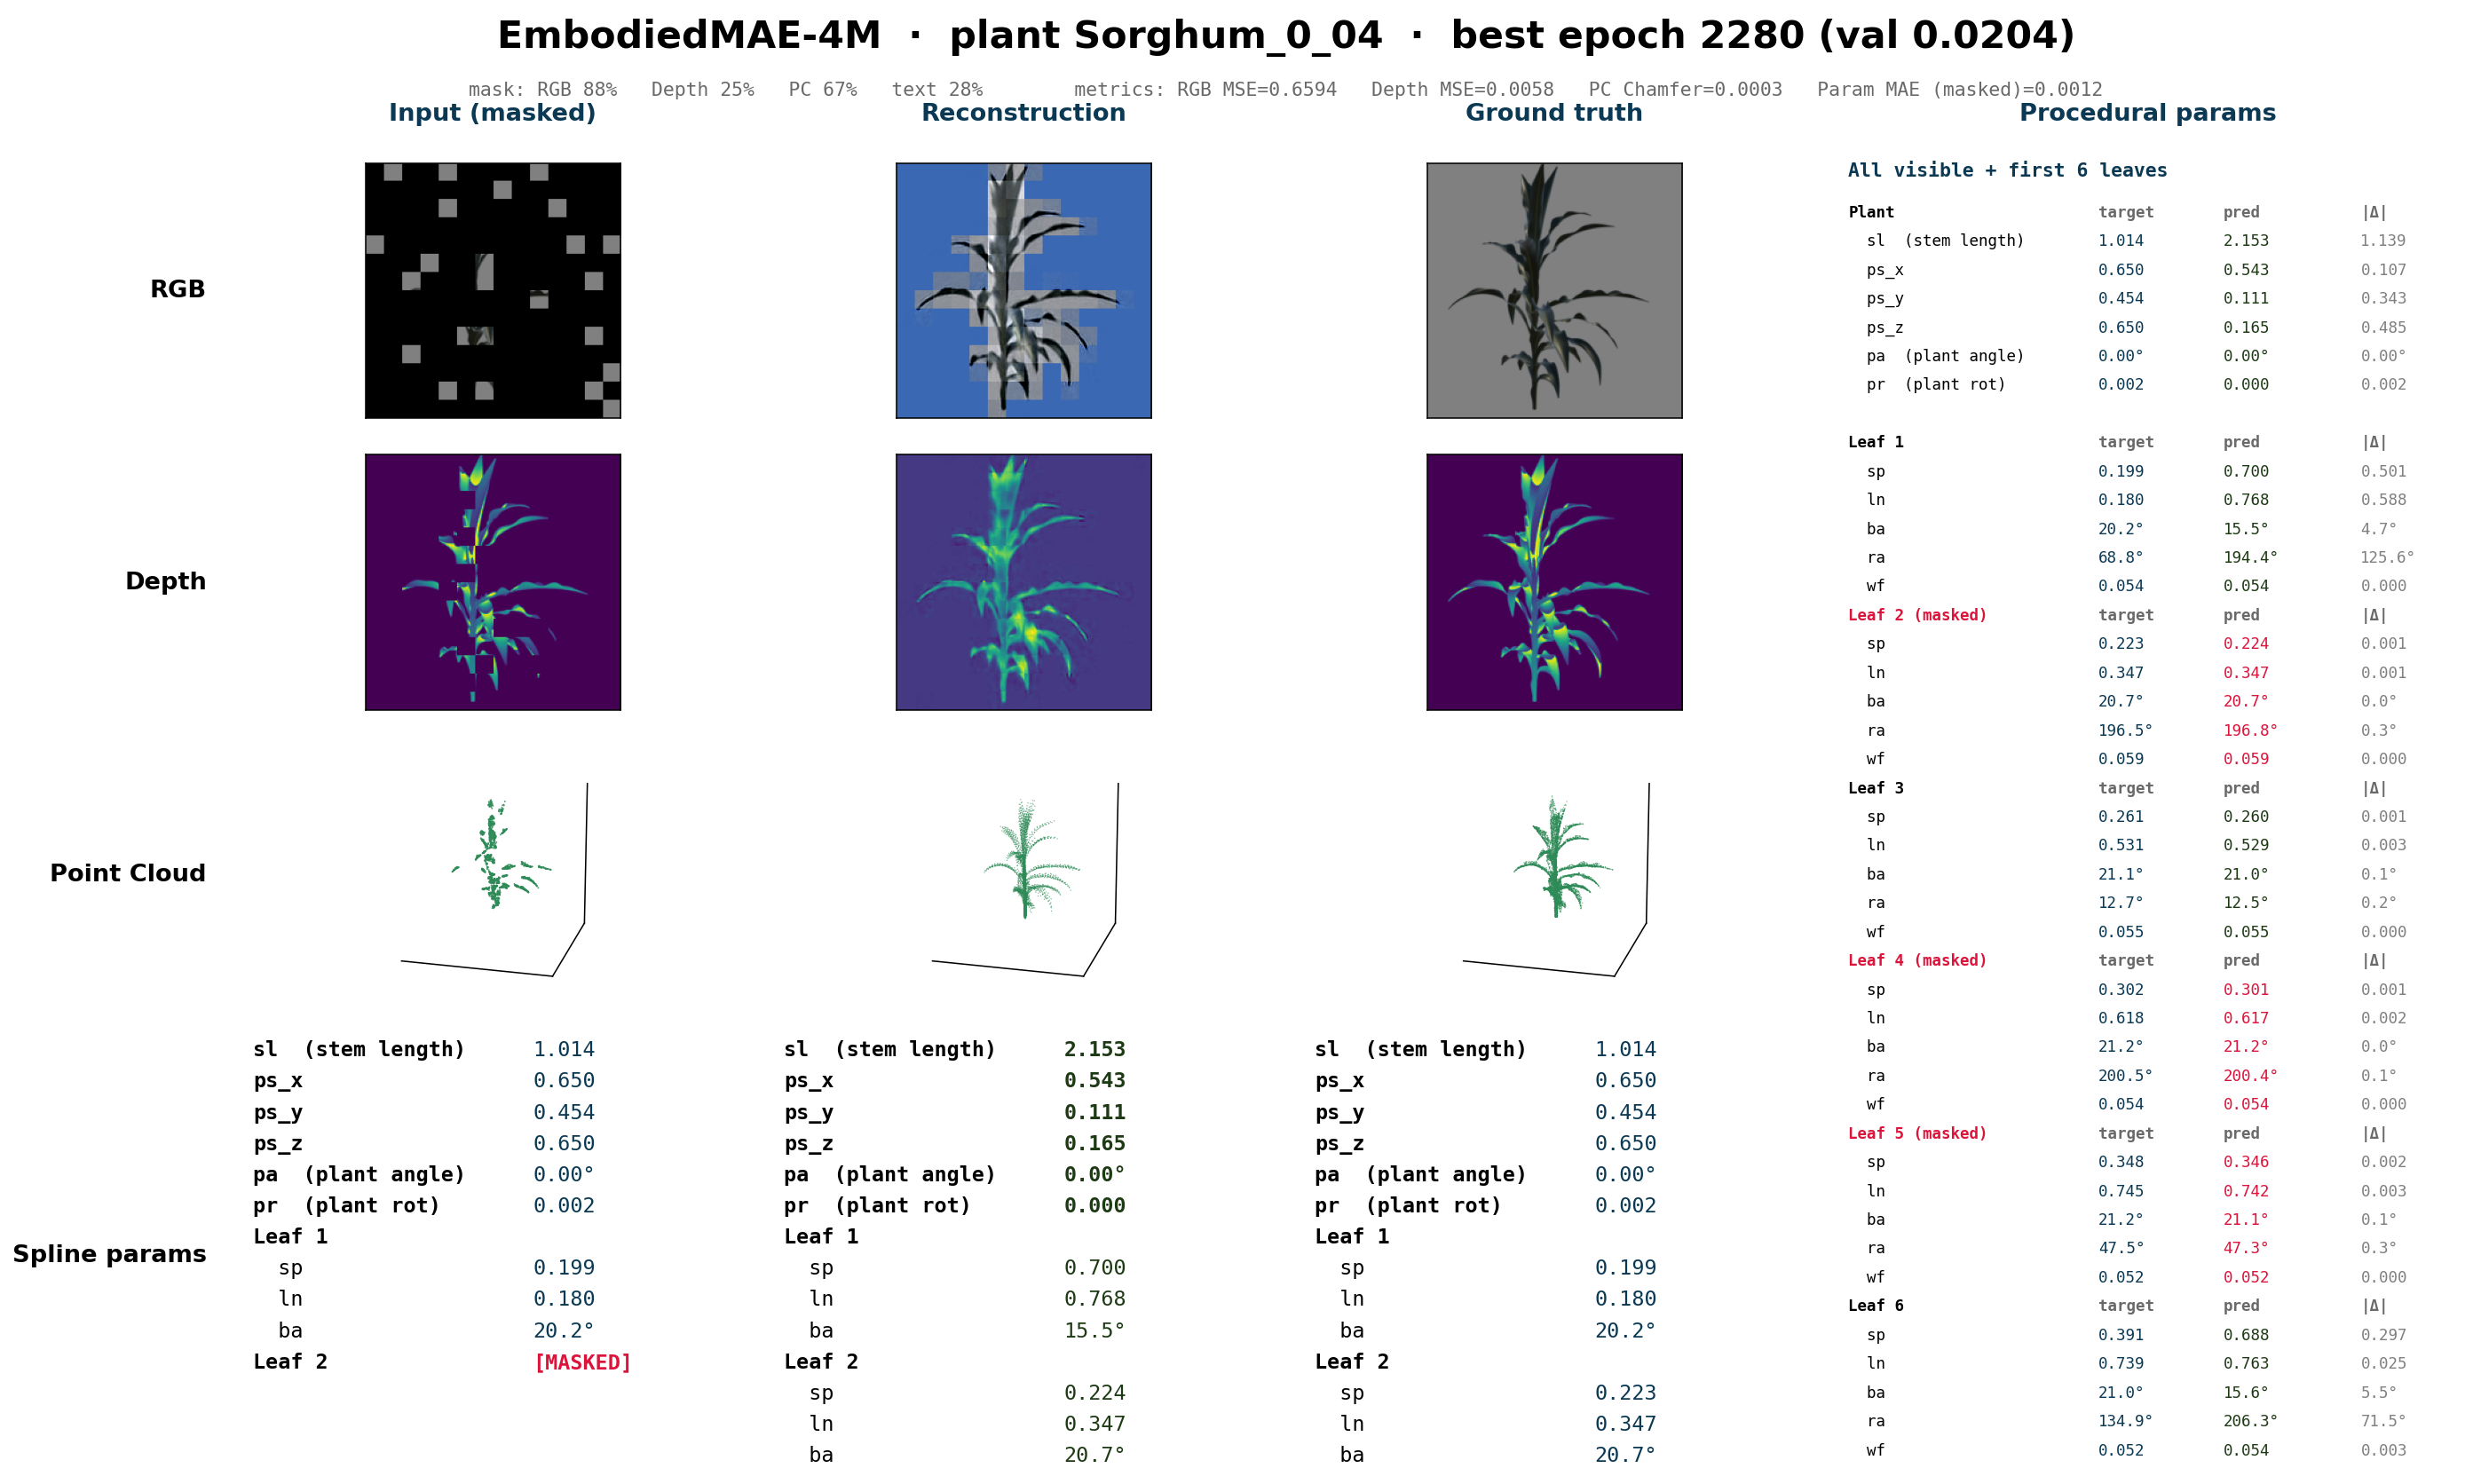
\includegraphics[width=\linewidth]{per_plant/Sorghum_0_04.png}
\caption{Plant Sorghum\_0\_04 -- epoch 2400 reconstruction.}
\label{fig:plant:Sorghum_0_04}
\end{figure}
\clearpage

\begin{figure}[H]
\centering
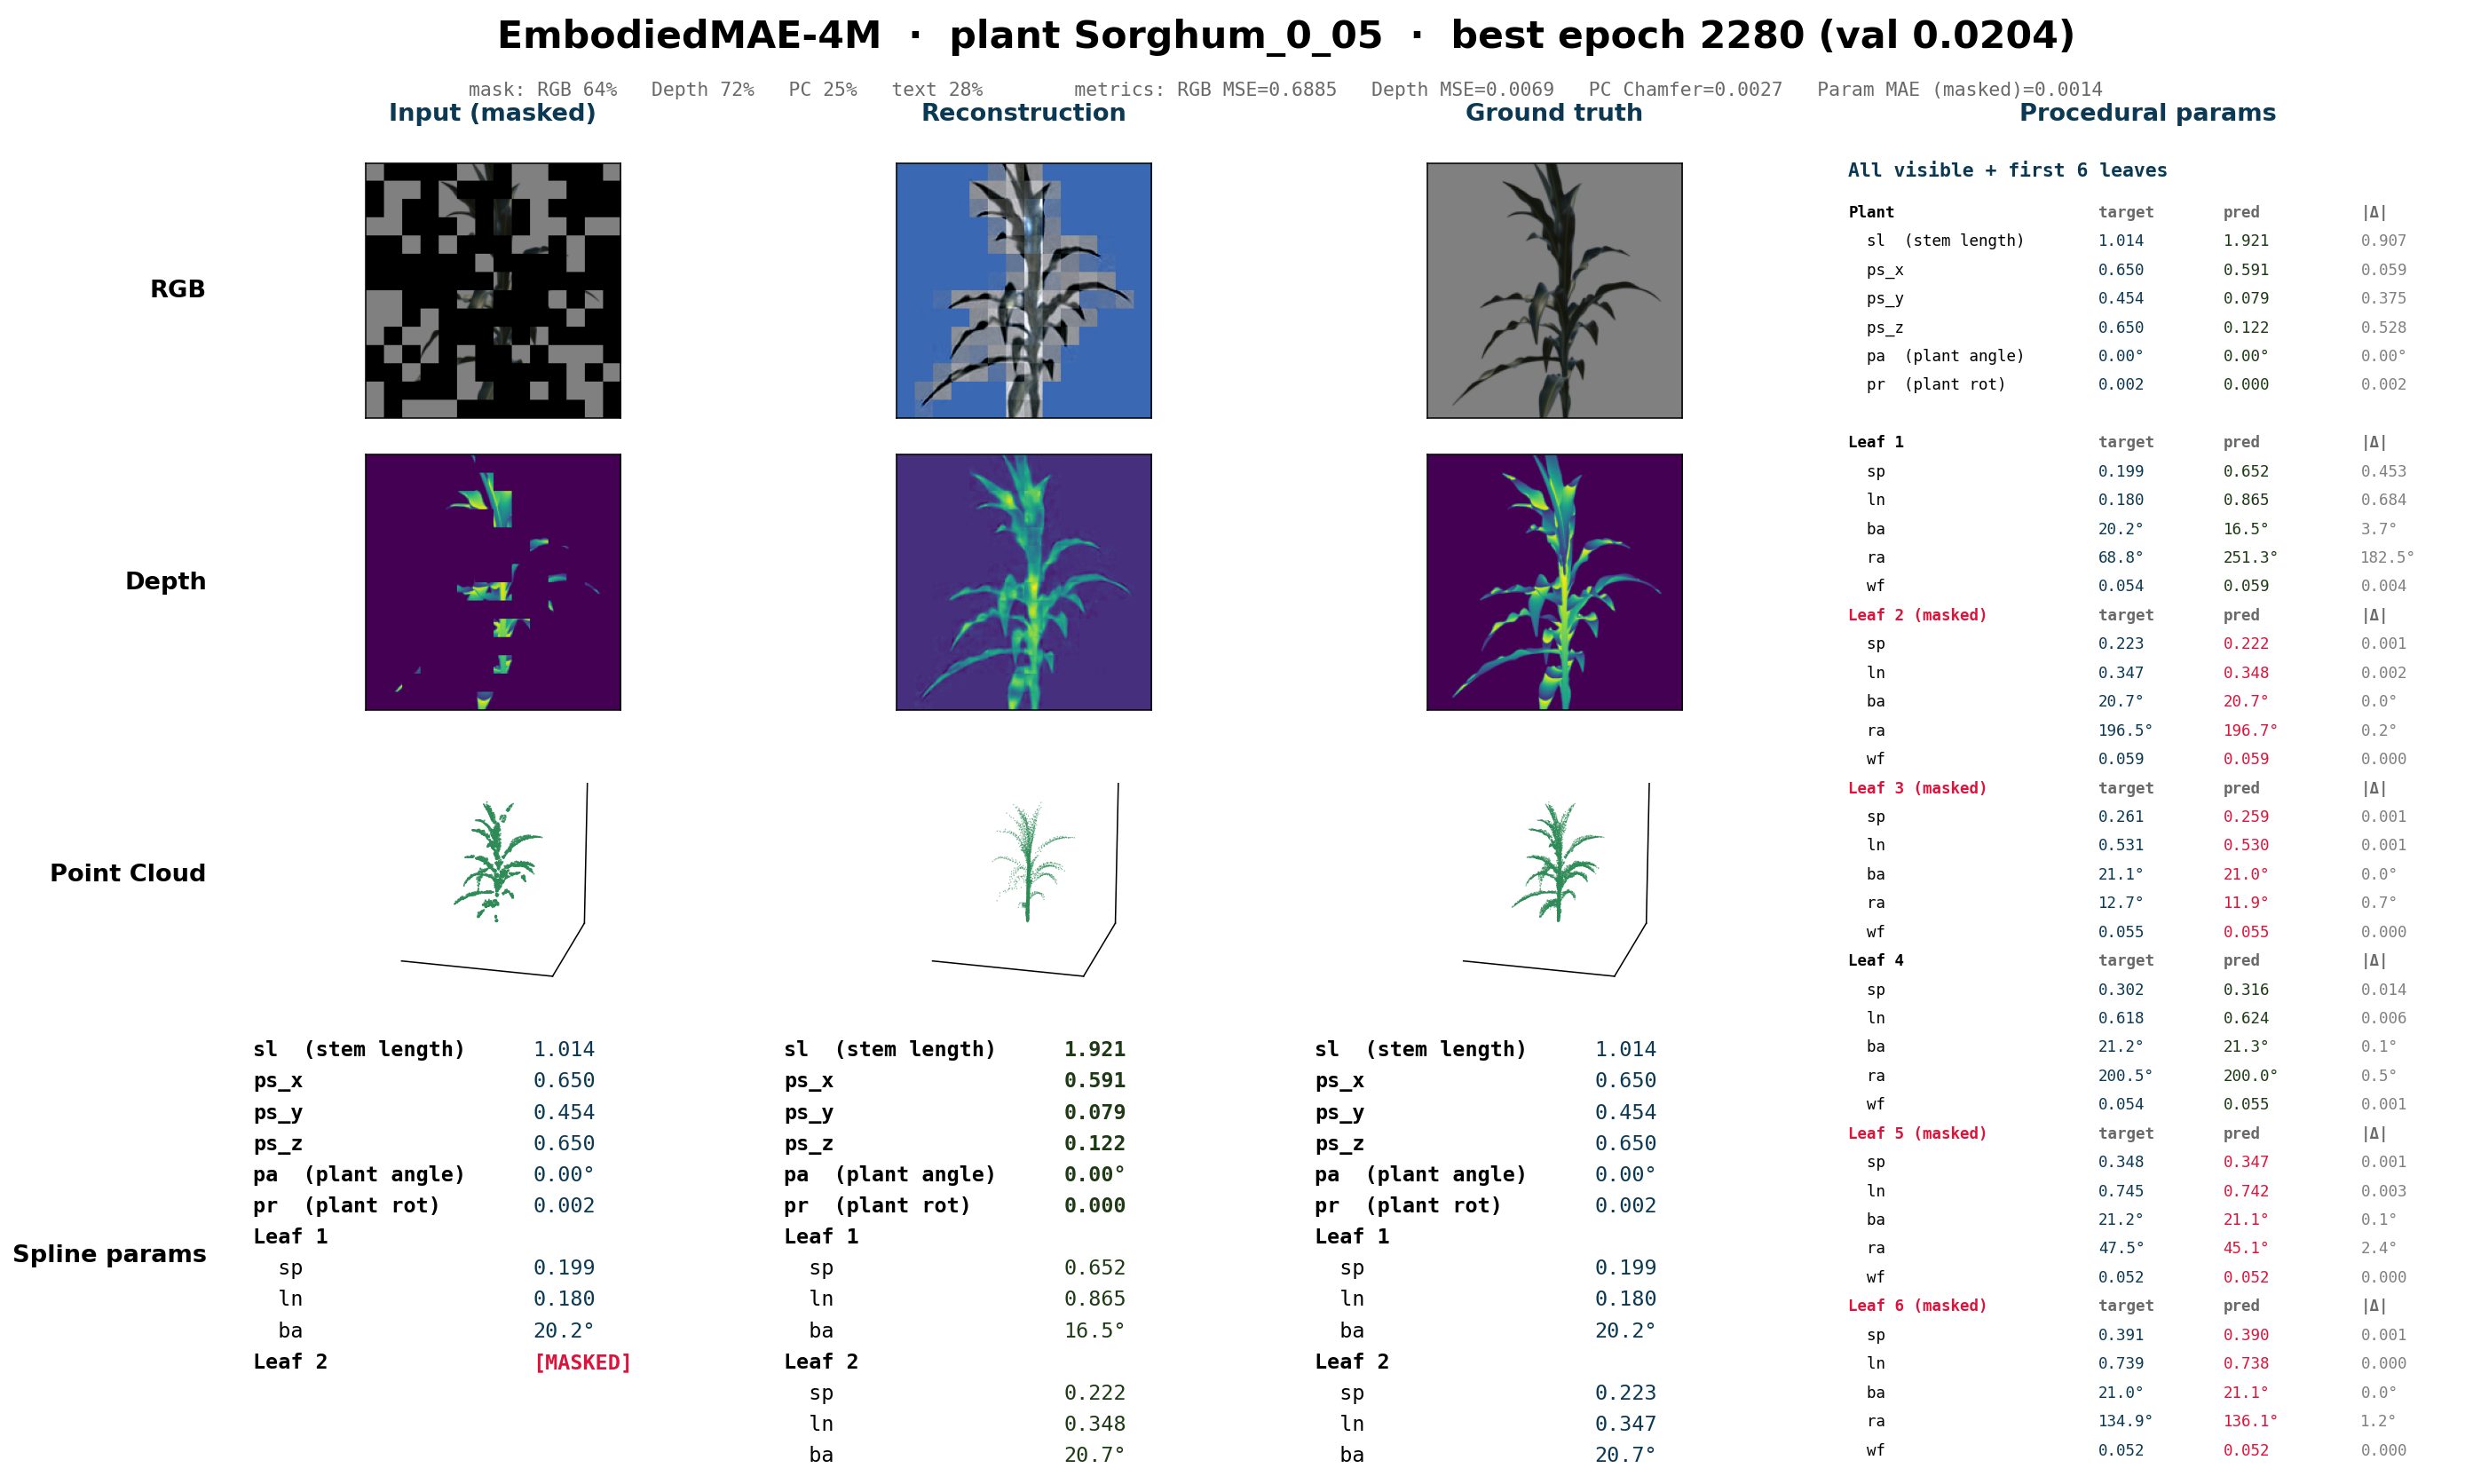
\includegraphics[width=\linewidth]{per_plant/Sorghum_0_05.png}
\caption{Plant Sorghum\_0\_05 -- epoch 2400 reconstruction.}
\label{fig:plant:Sorghum_0_05}
\end{figure}
\clearpage

\begin{figure}[H]
\centering
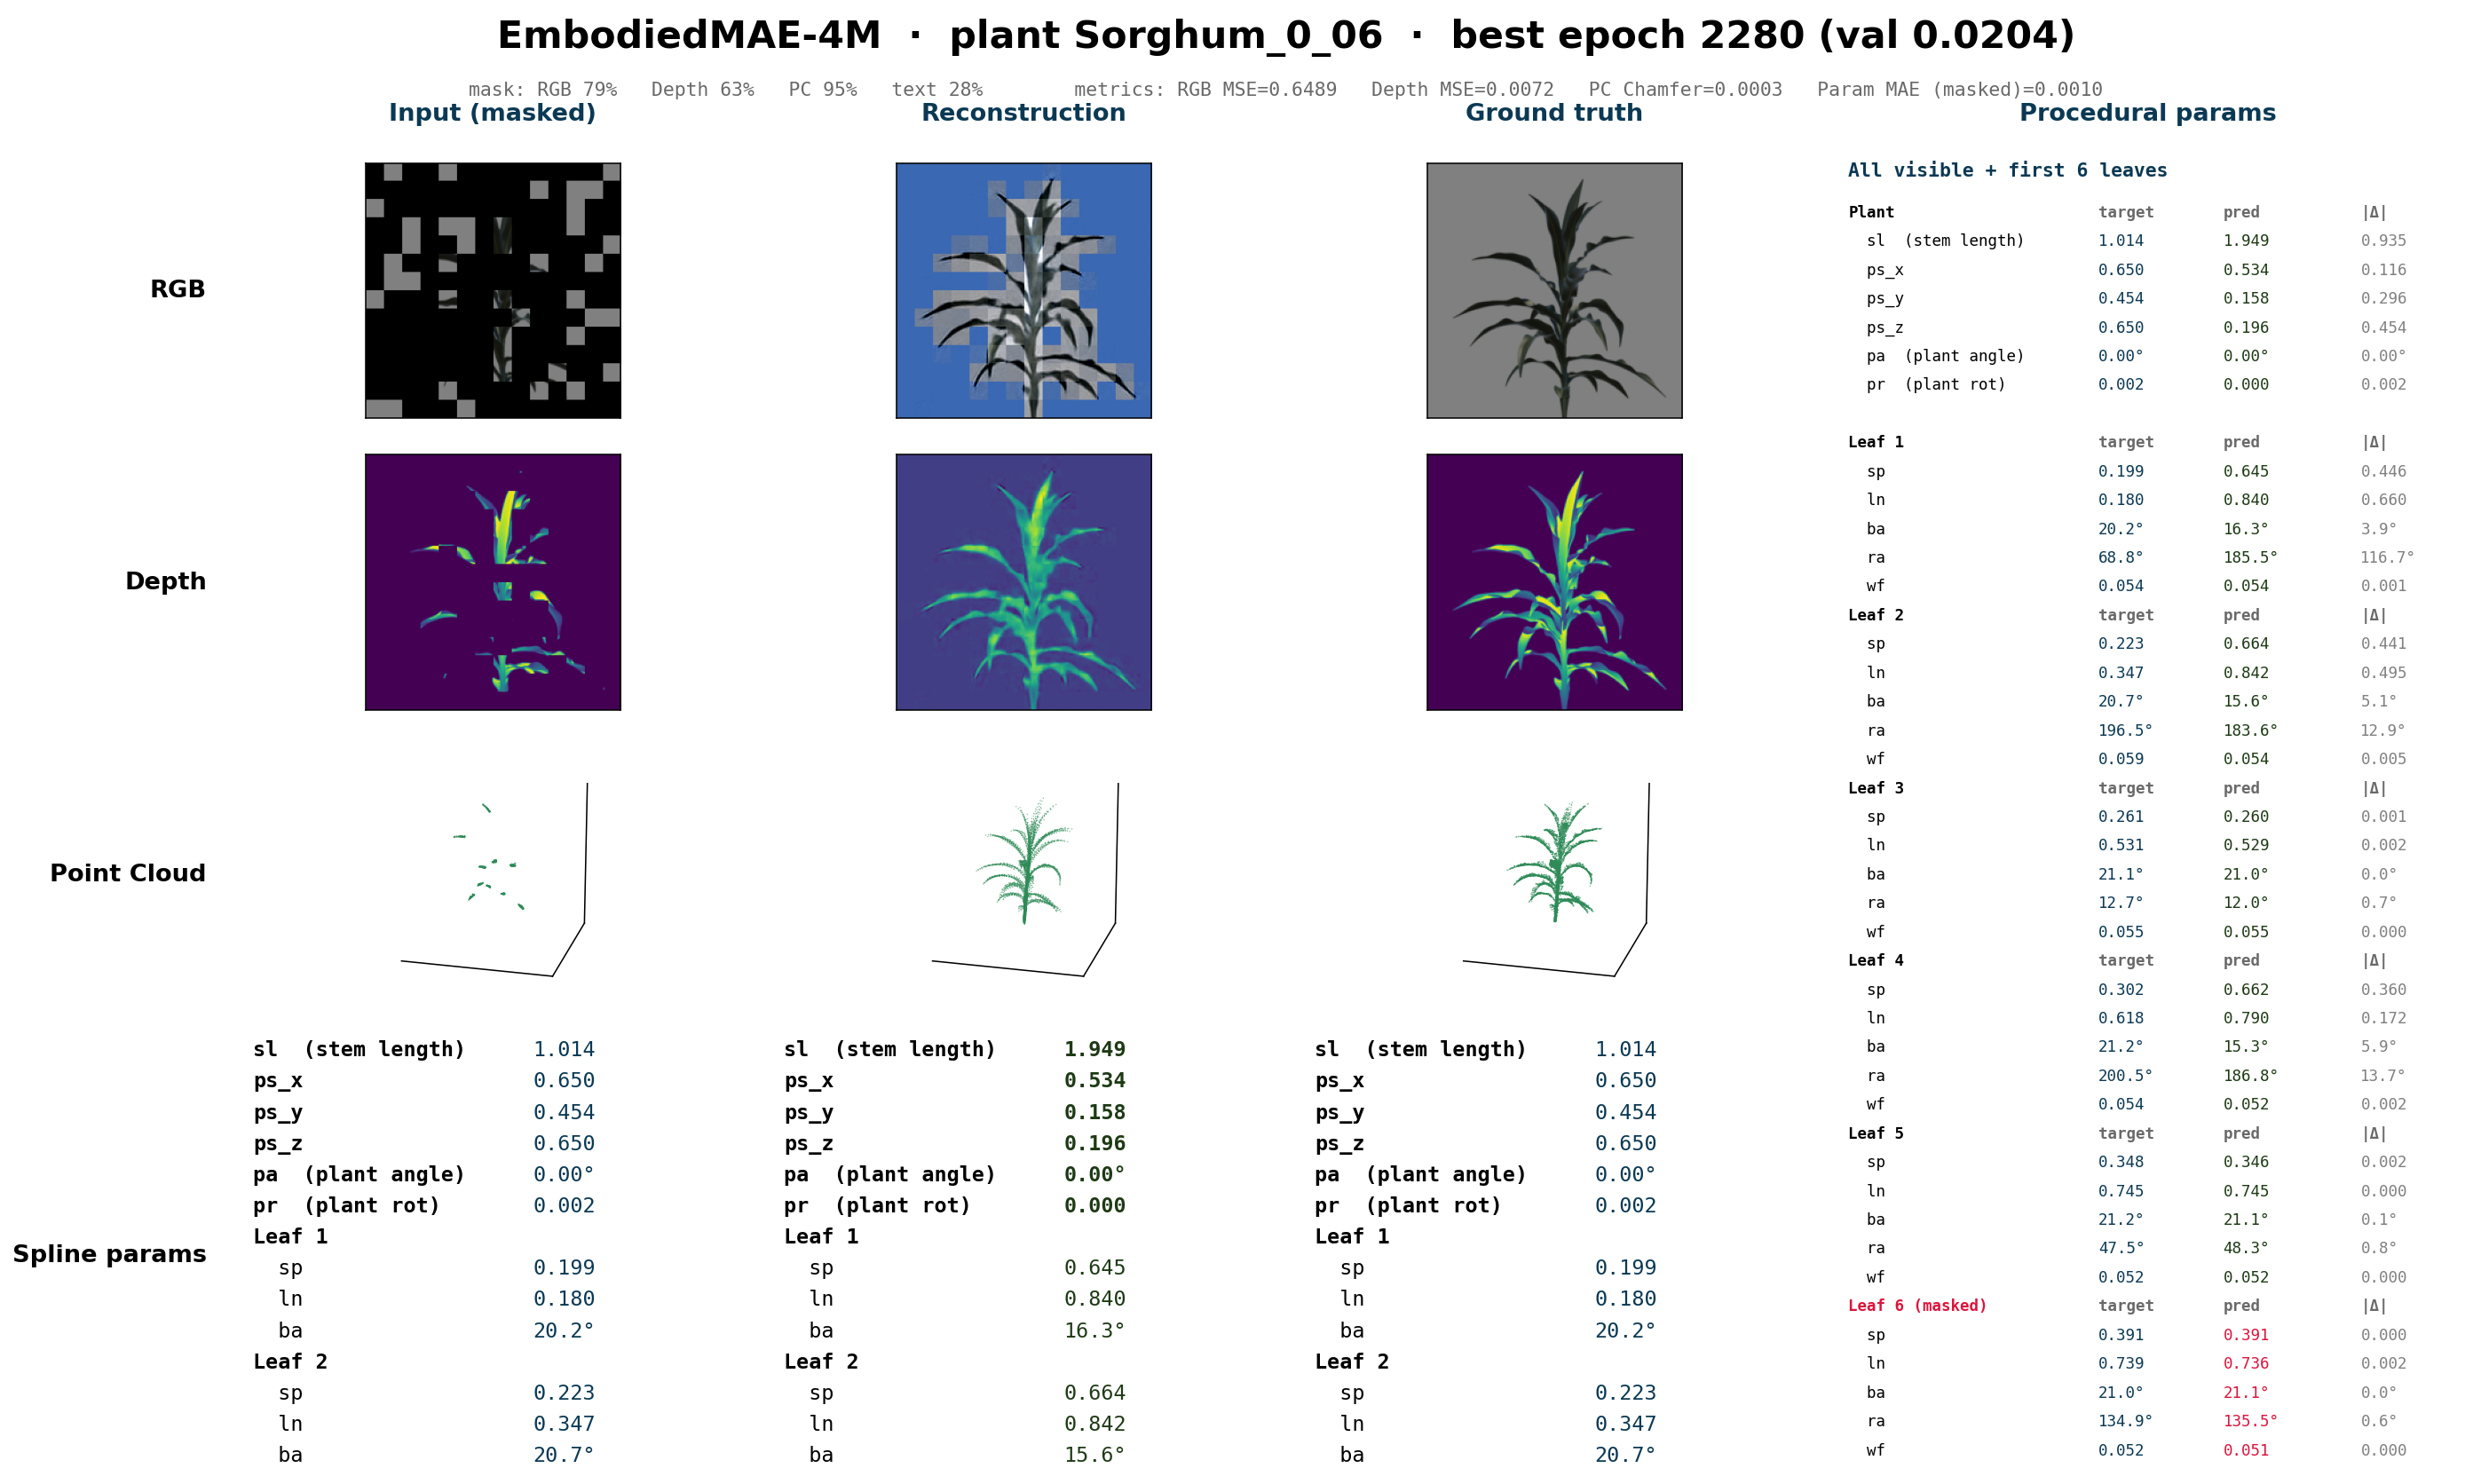
\includegraphics[width=\linewidth]{per_plant/Sorghum_0_06.png}
\caption{Plant Sorghum\_0\_06 -- epoch 2400 reconstruction.}
\label{fig:plant:Sorghum_0_06}
\end{figure}
\clearpage

\begin{figure}[H]
\centering
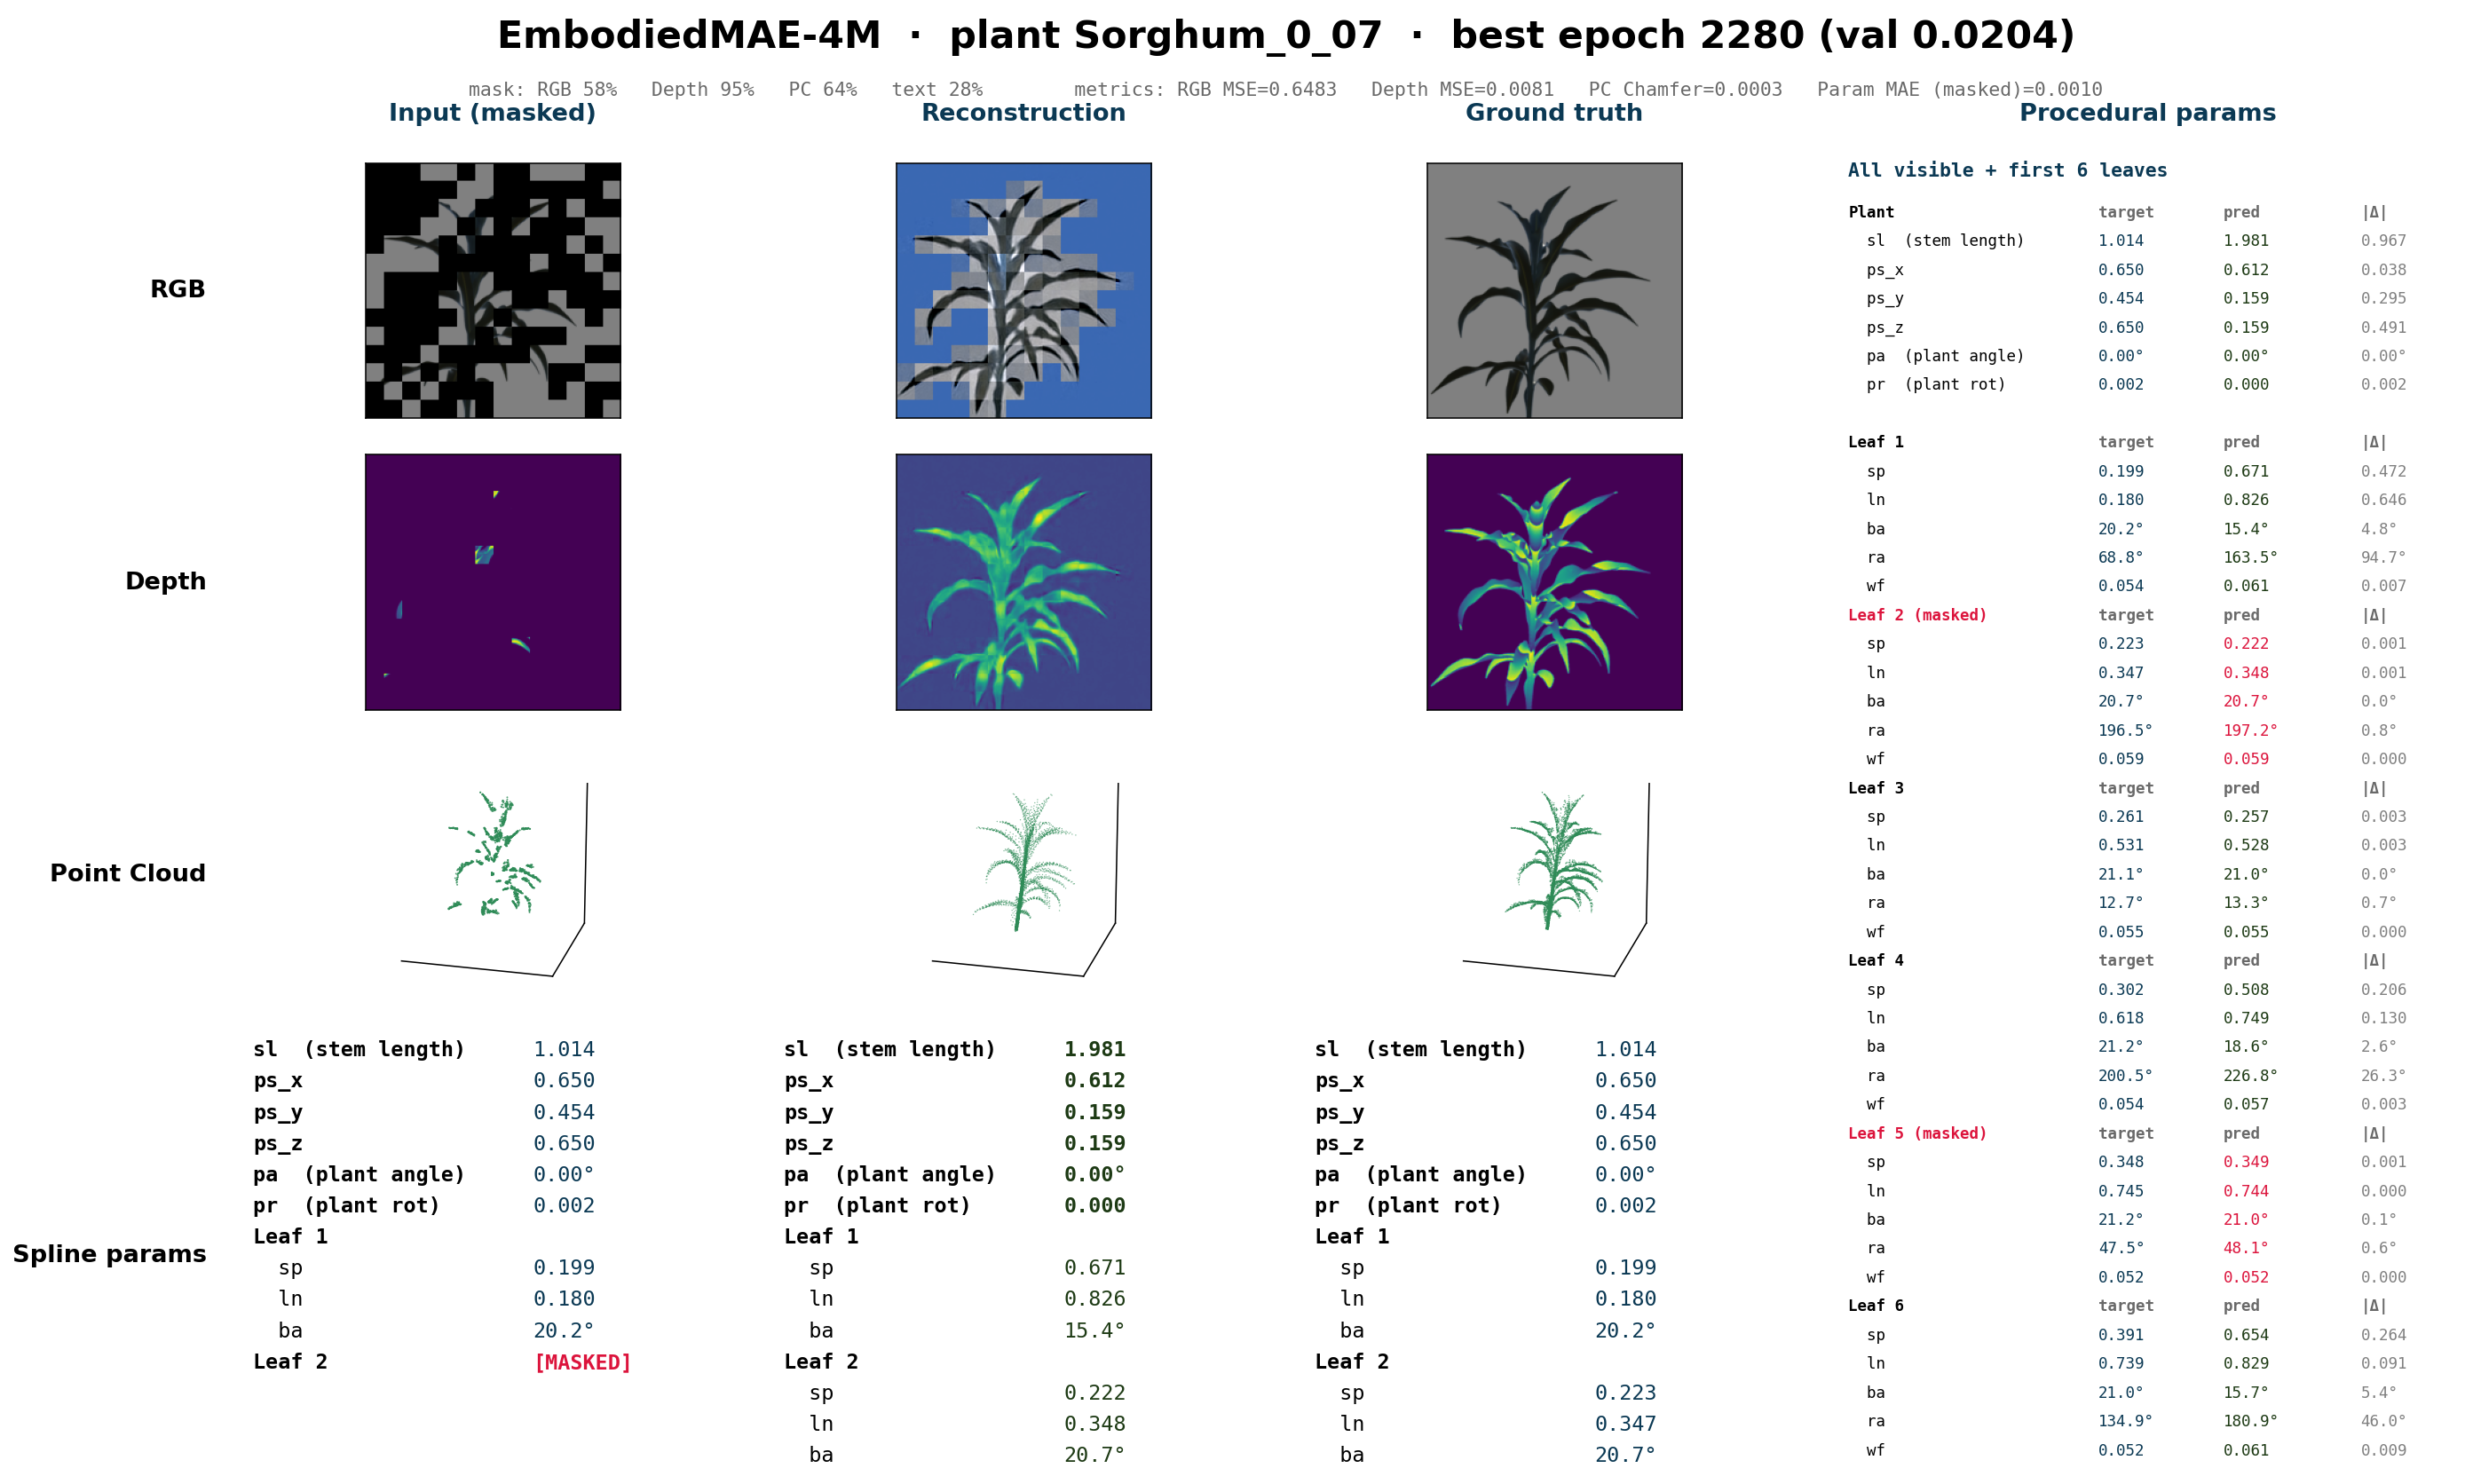
\includegraphics[width=\linewidth]{per_plant/Sorghum_0_07.png}
\caption{Plant Sorghum\_0\_07 -- epoch 2400 reconstruction.}
\label{fig:plant:Sorghum_0_07}
\end{figure}
\clearpage

\begin{figure}[H]
\centering
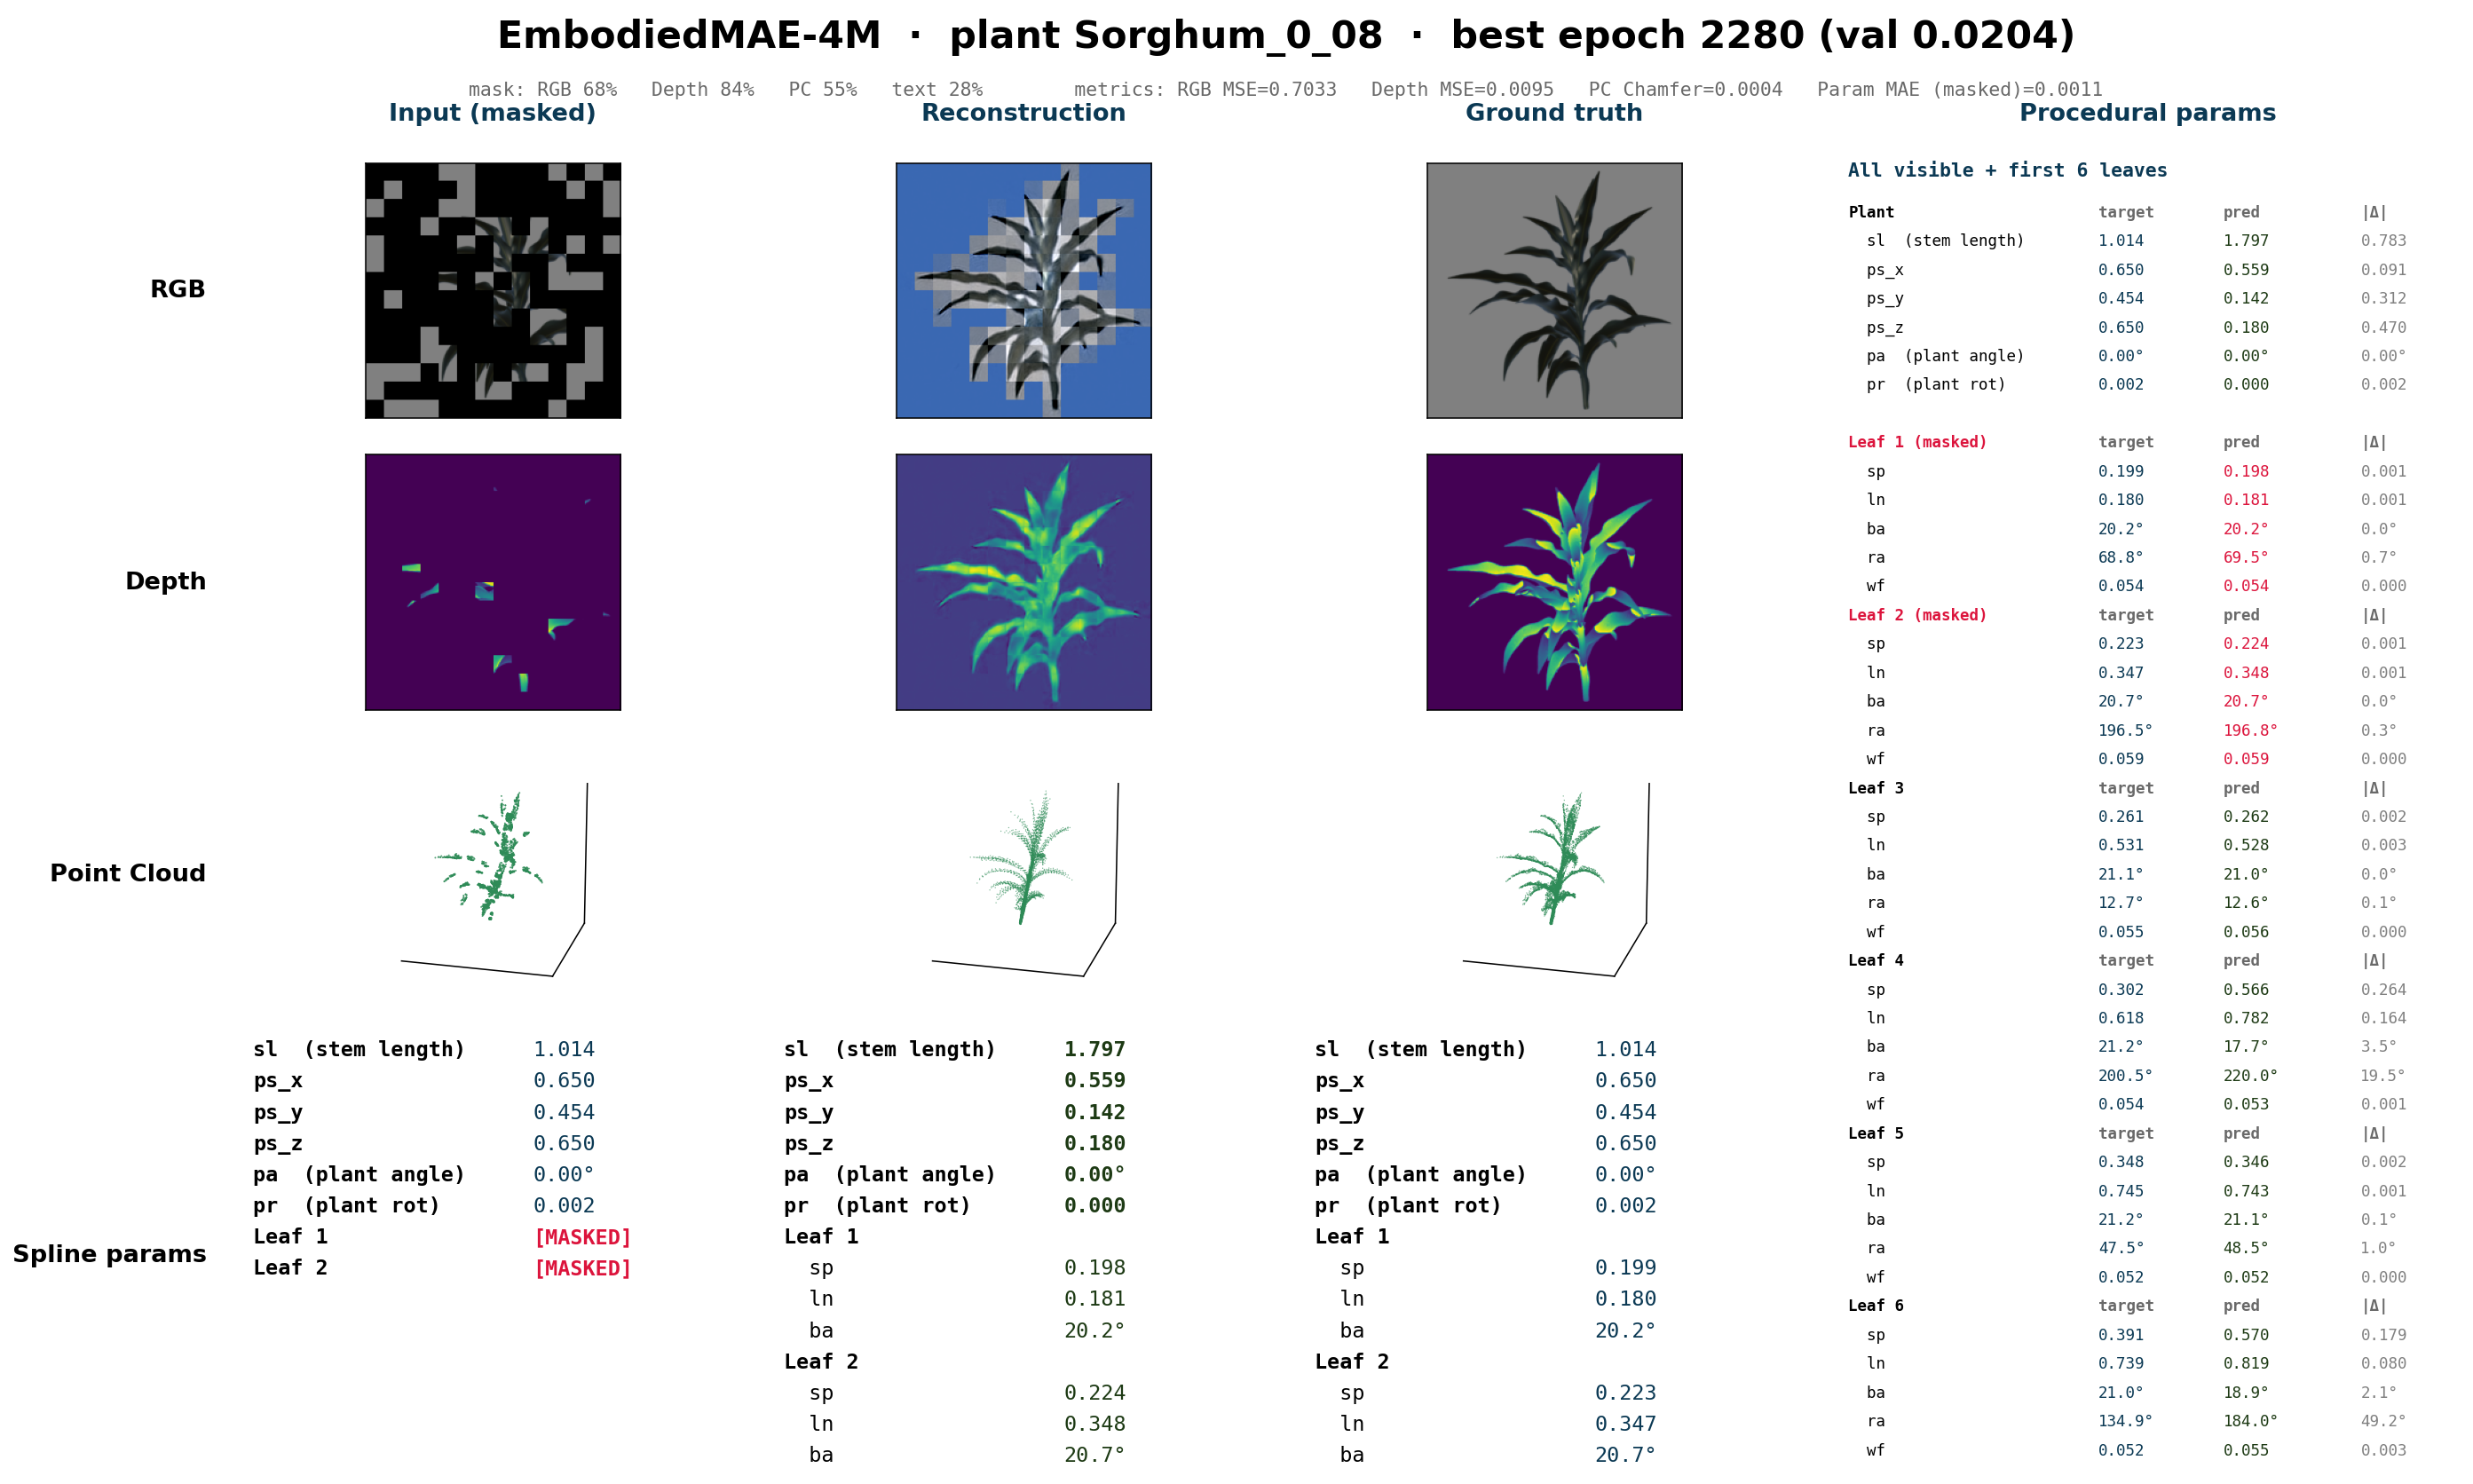
\includegraphics[width=\linewidth]{per_plant/Sorghum_0_08.png}
\caption{Plant Sorghum\_0\_08 -- epoch 2400 reconstruction.}
\label{fig:plant:Sorghum_0_08}
\end{figure}
\clearpage

\begin{figure}[H]
\centering
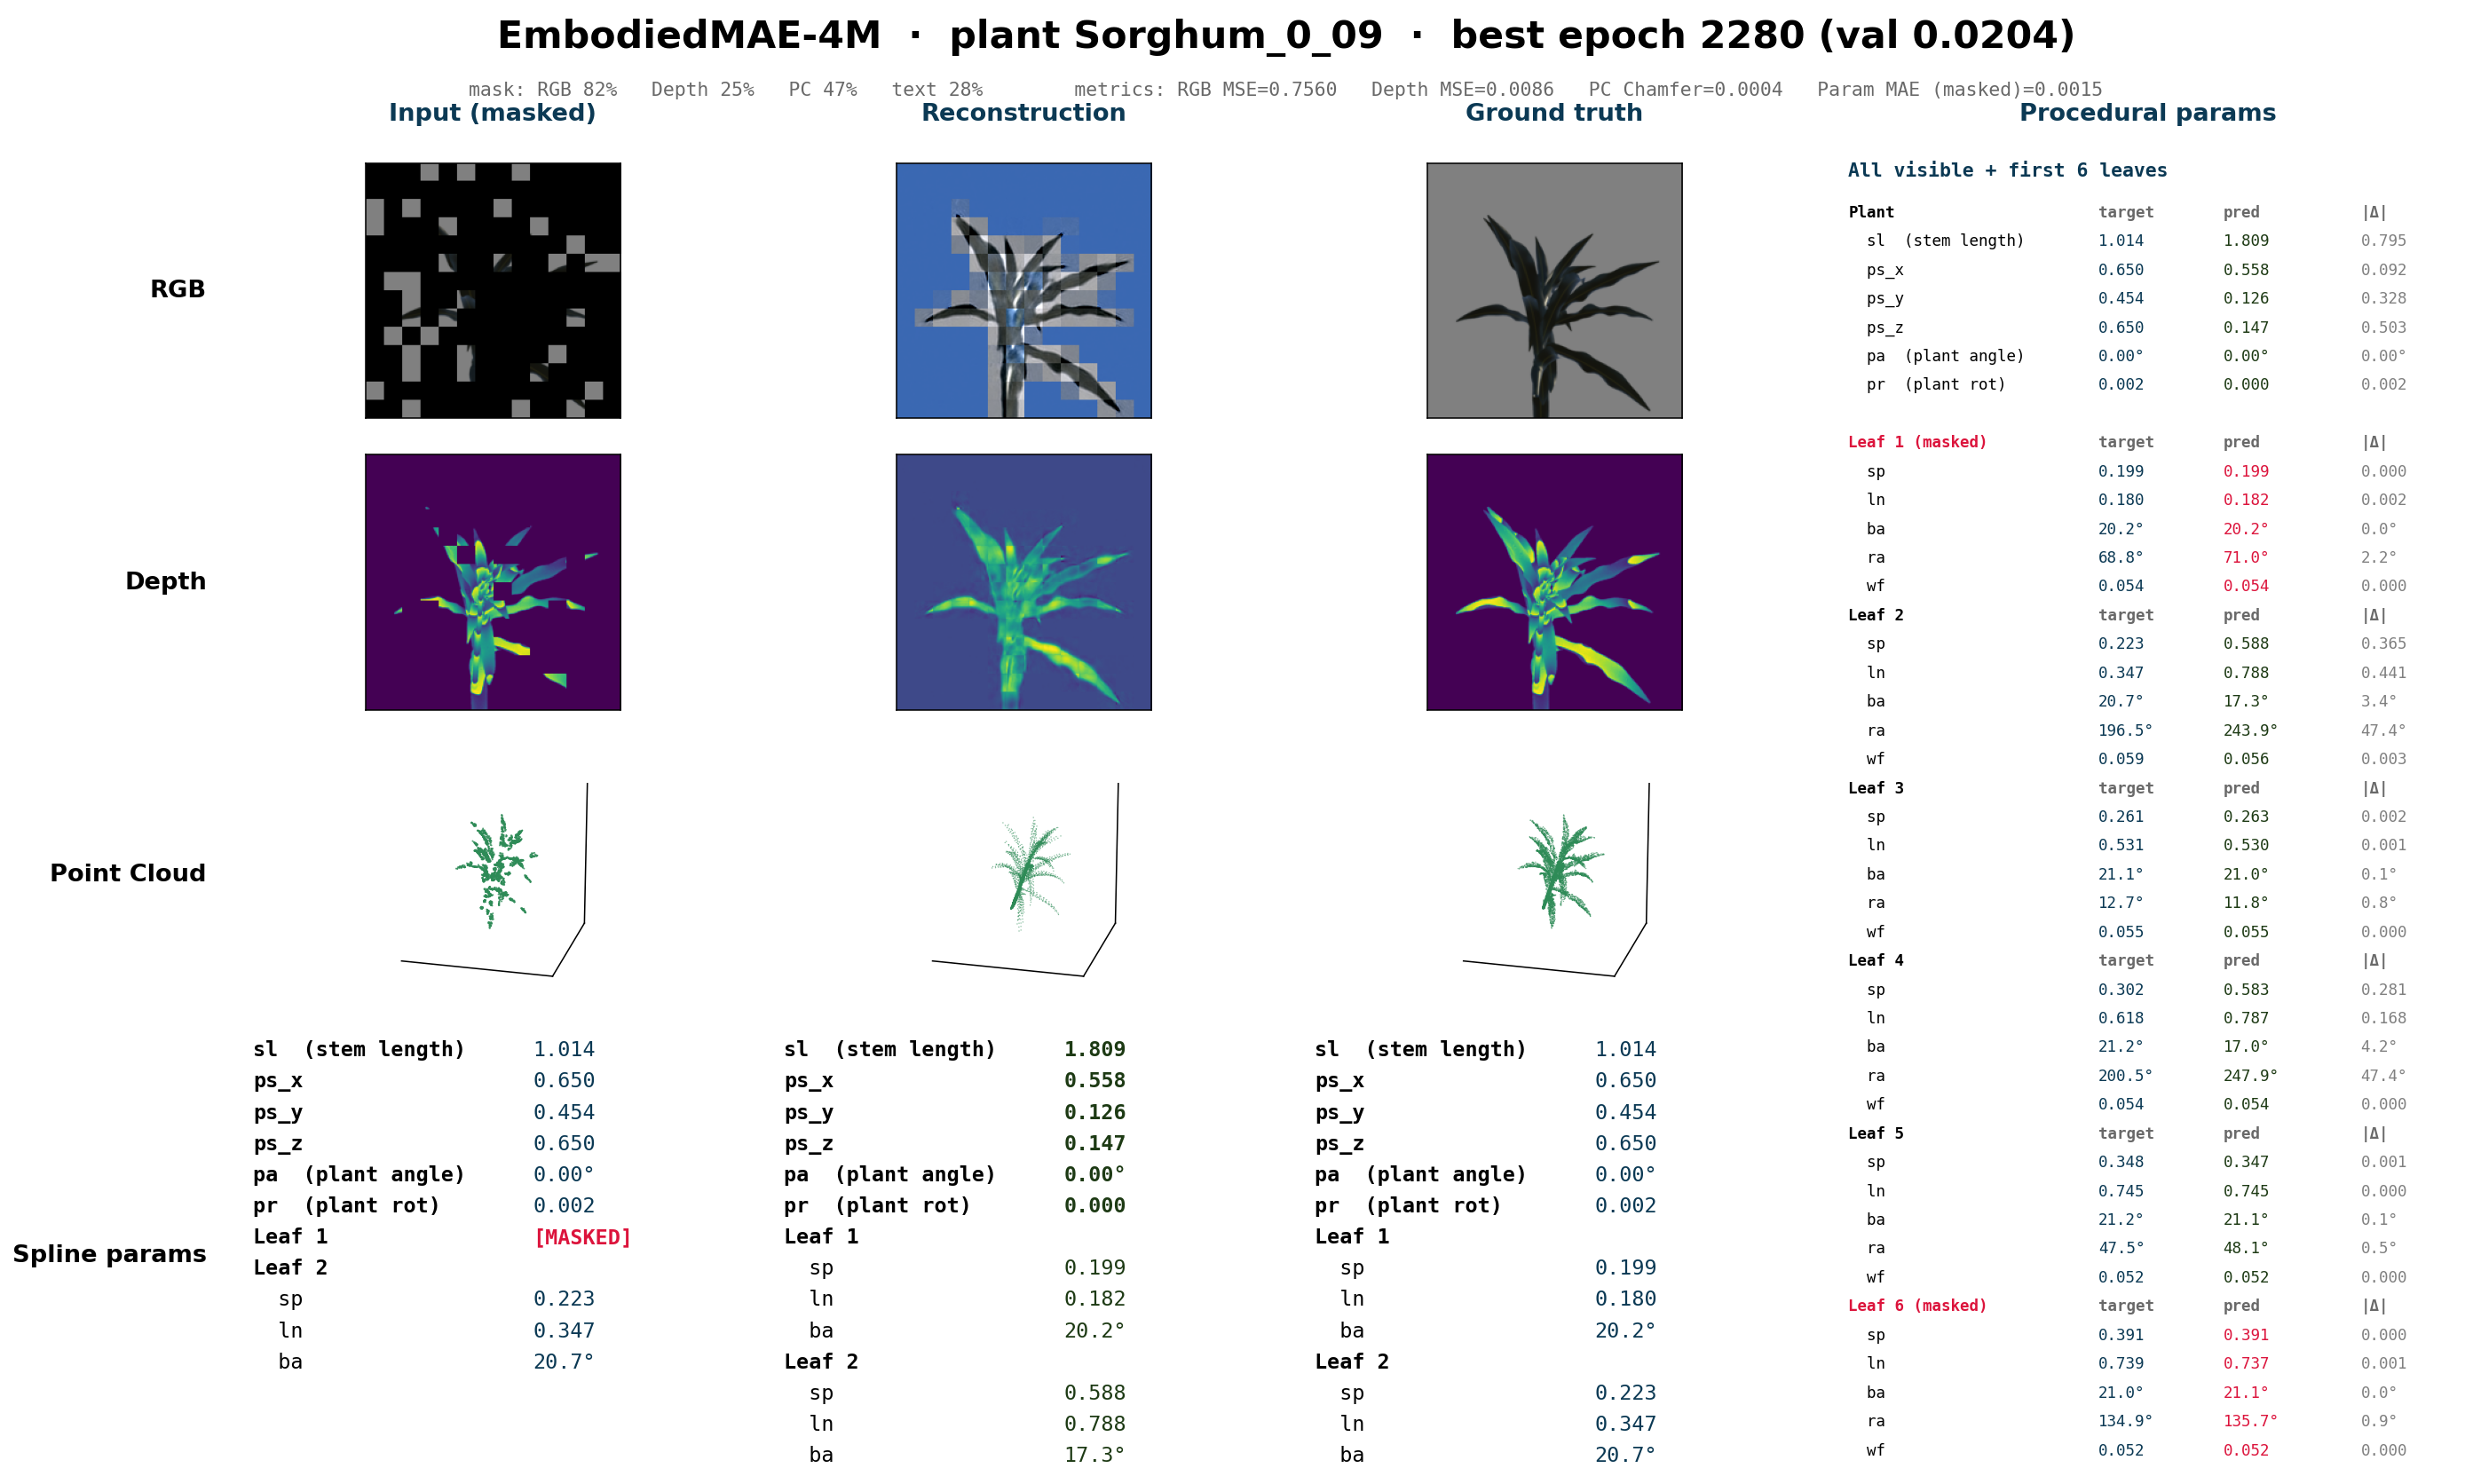
\includegraphics[width=\linewidth]{per_plant/Sorghum_0_09.png}
\caption{Plant Sorghum\_0\_09 -- epoch 2400 reconstruction.}
\label{fig:plant:Sorghum_0_09}
\end{figure}
\clearpage

\begin{figure}[H]
\centering
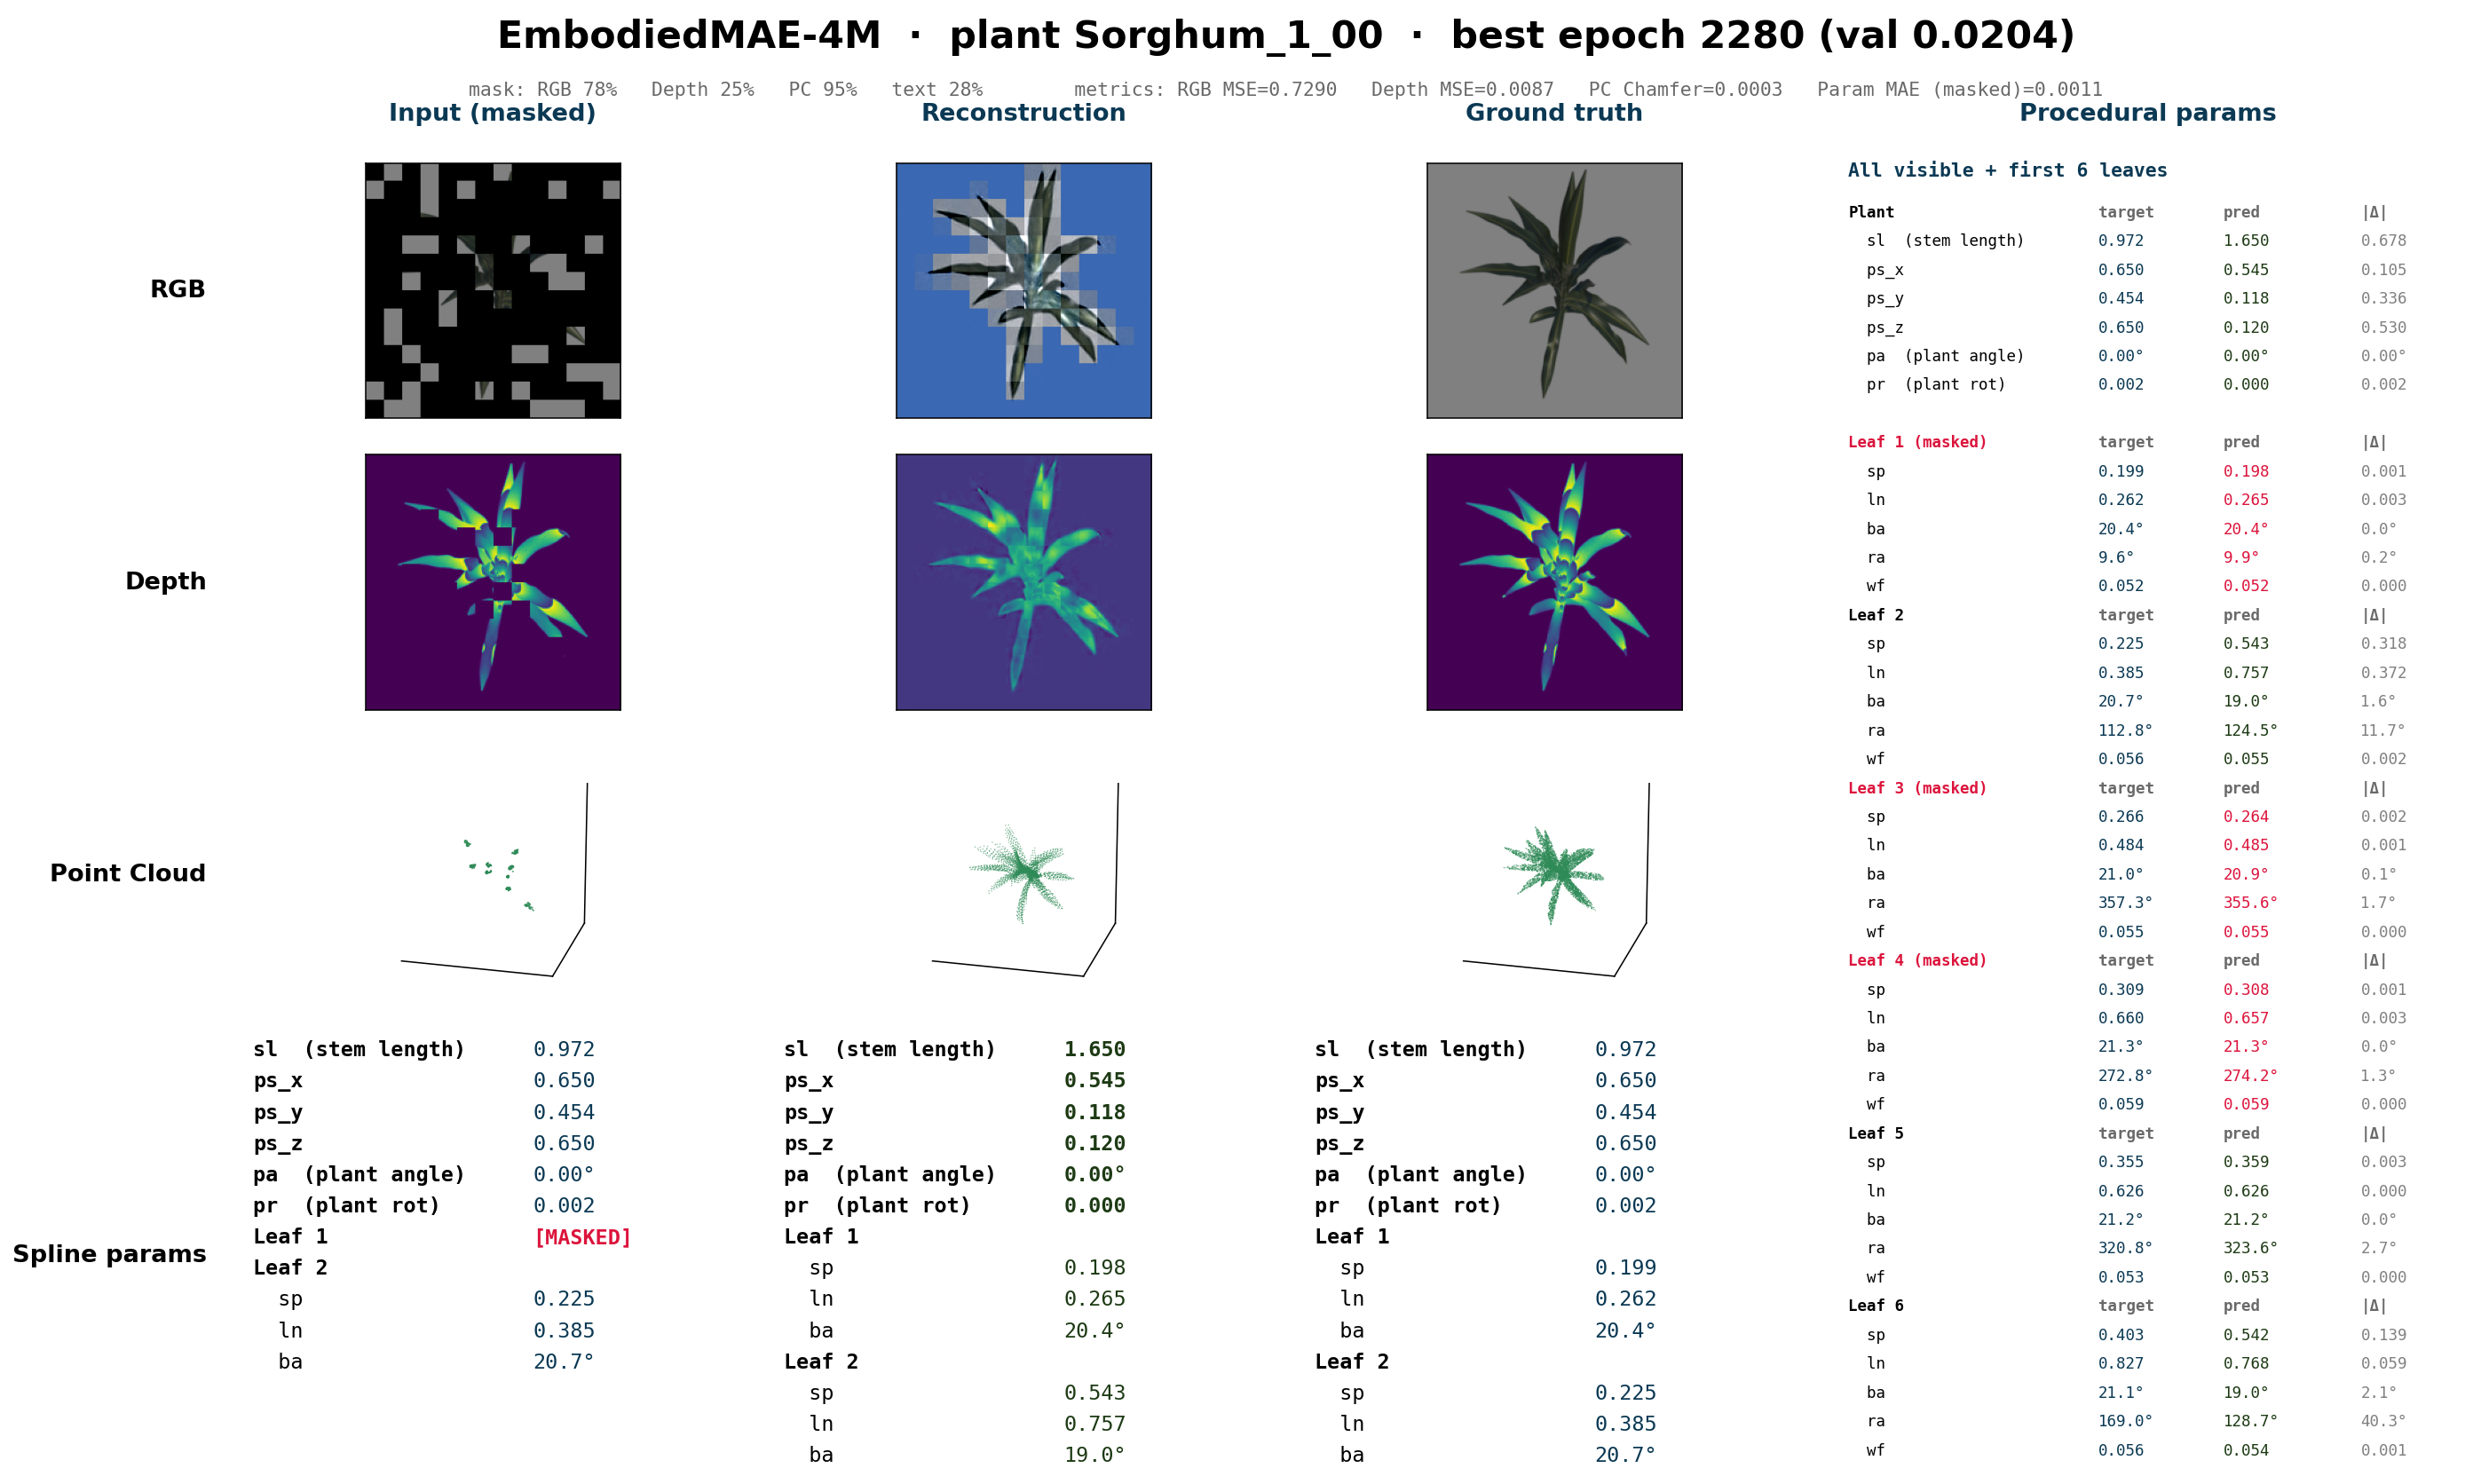
\includegraphics[width=\linewidth]{per_plant/Sorghum_1_00.png}
\caption{Plant Sorghum\_1\_00 -- epoch 2400 reconstruction.}
\label{fig:plant:Sorghum_1_00}
\end{figure}
\clearpage

\begin{figure}[H]
\centering
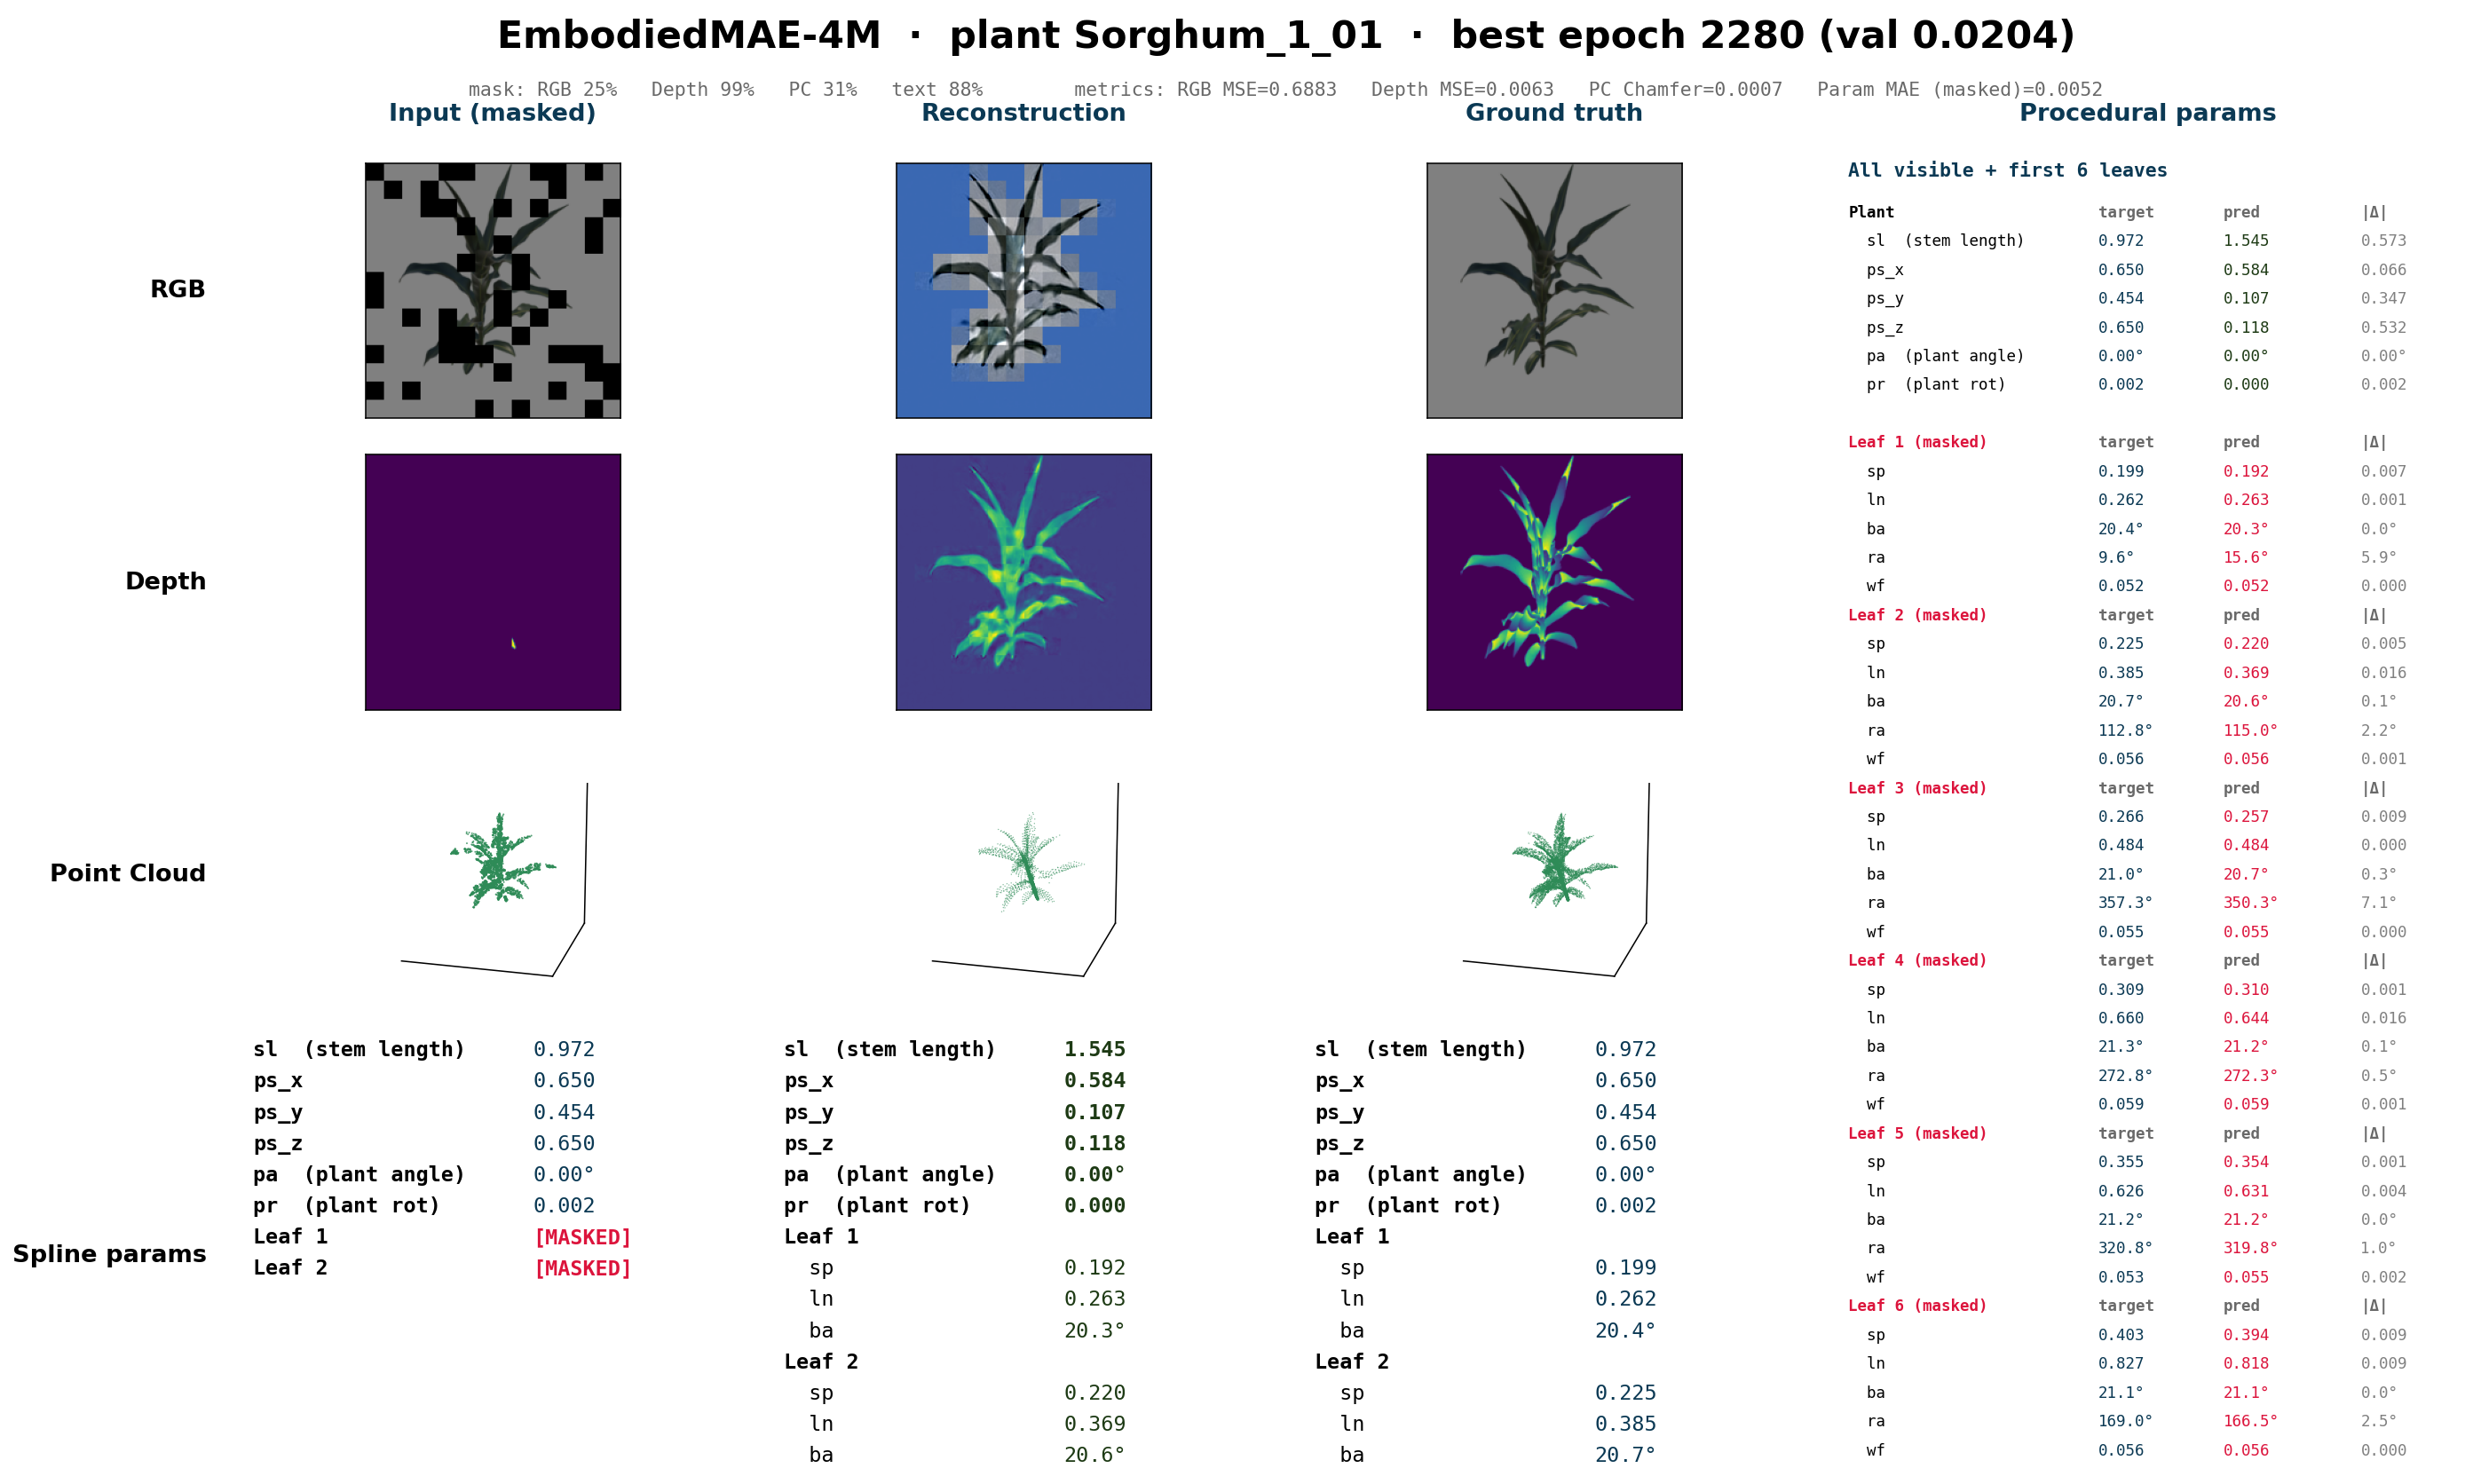
\includegraphics[width=\linewidth]{per_plant/Sorghum_1_01.png}
\caption{Plant Sorghum\_1\_01 -- epoch 2400 reconstruction.}
\label{fig:plant:Sorghum_1_01}
\end{figure}
\clearpage

\begin{figure}[H]
\centering
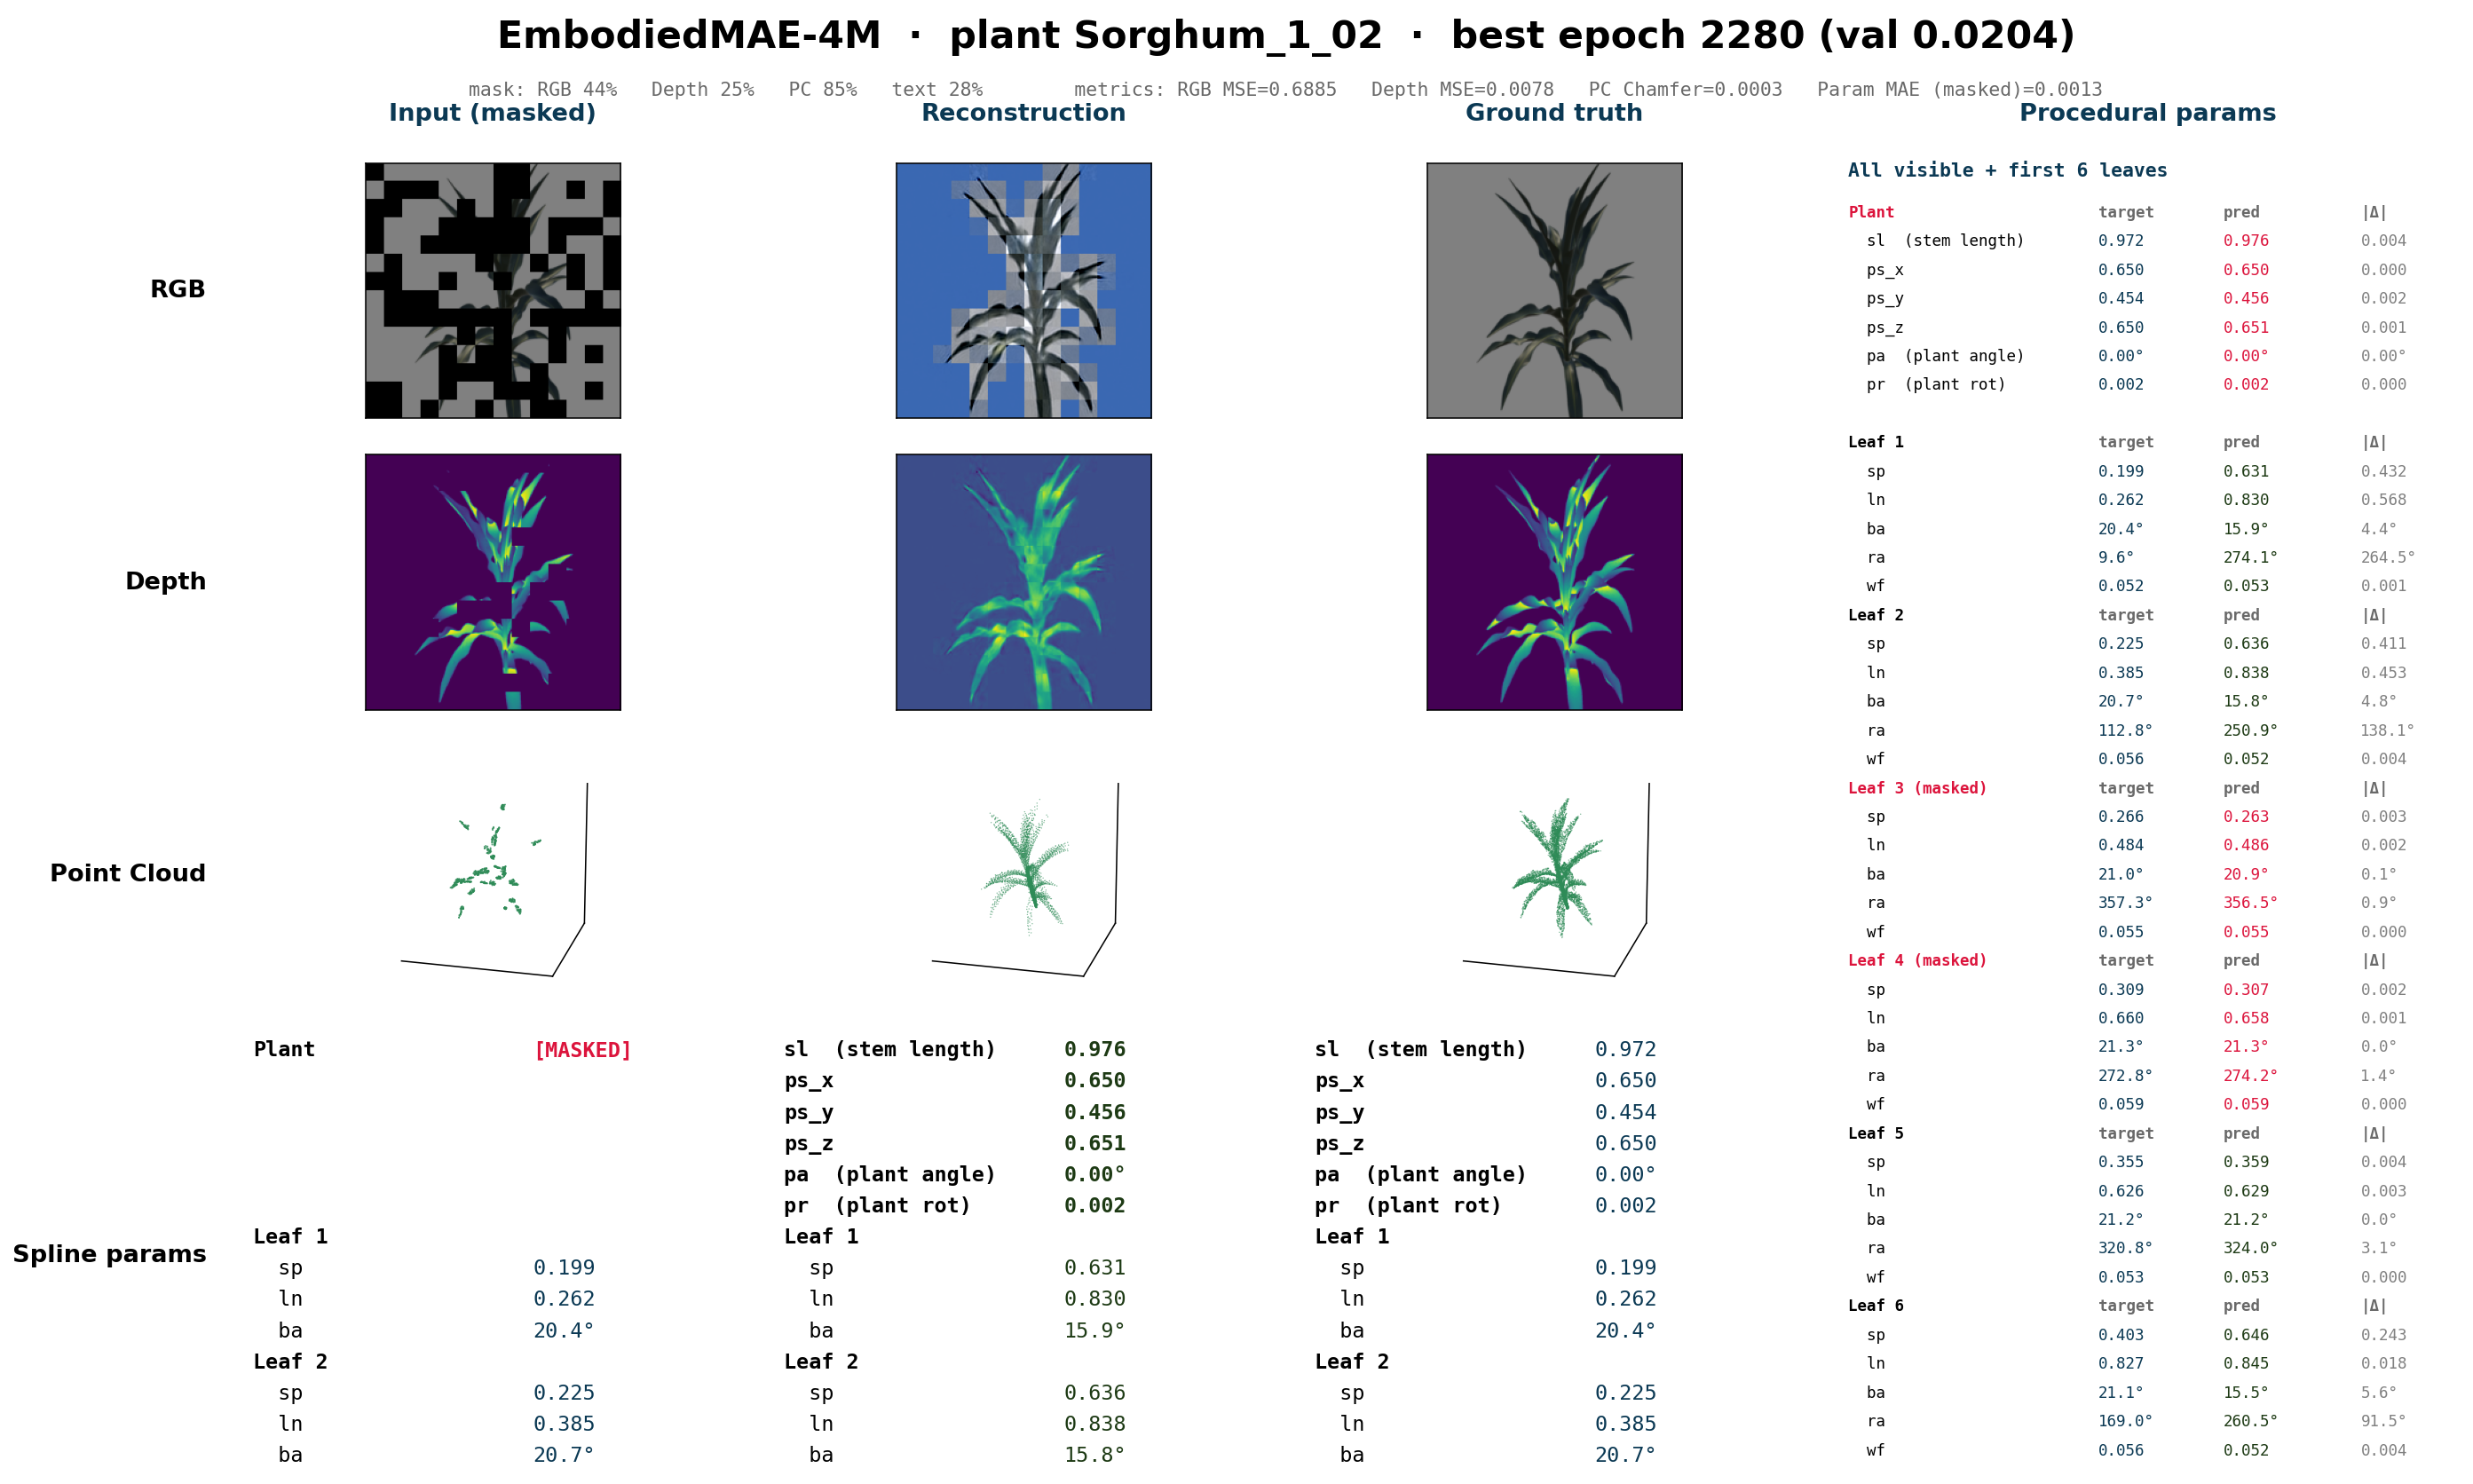
\includegraphics[width=\linewidth]{per_plant/Sorghum_1_02.png}
\caption{Plant Sorghum\_1\_02 -- epoch 2400 reconstruction.}
\label{fig:plant:Sorghum_1_02}
\end{figure}
\clearpage

\begin{figure}[H]
\centering
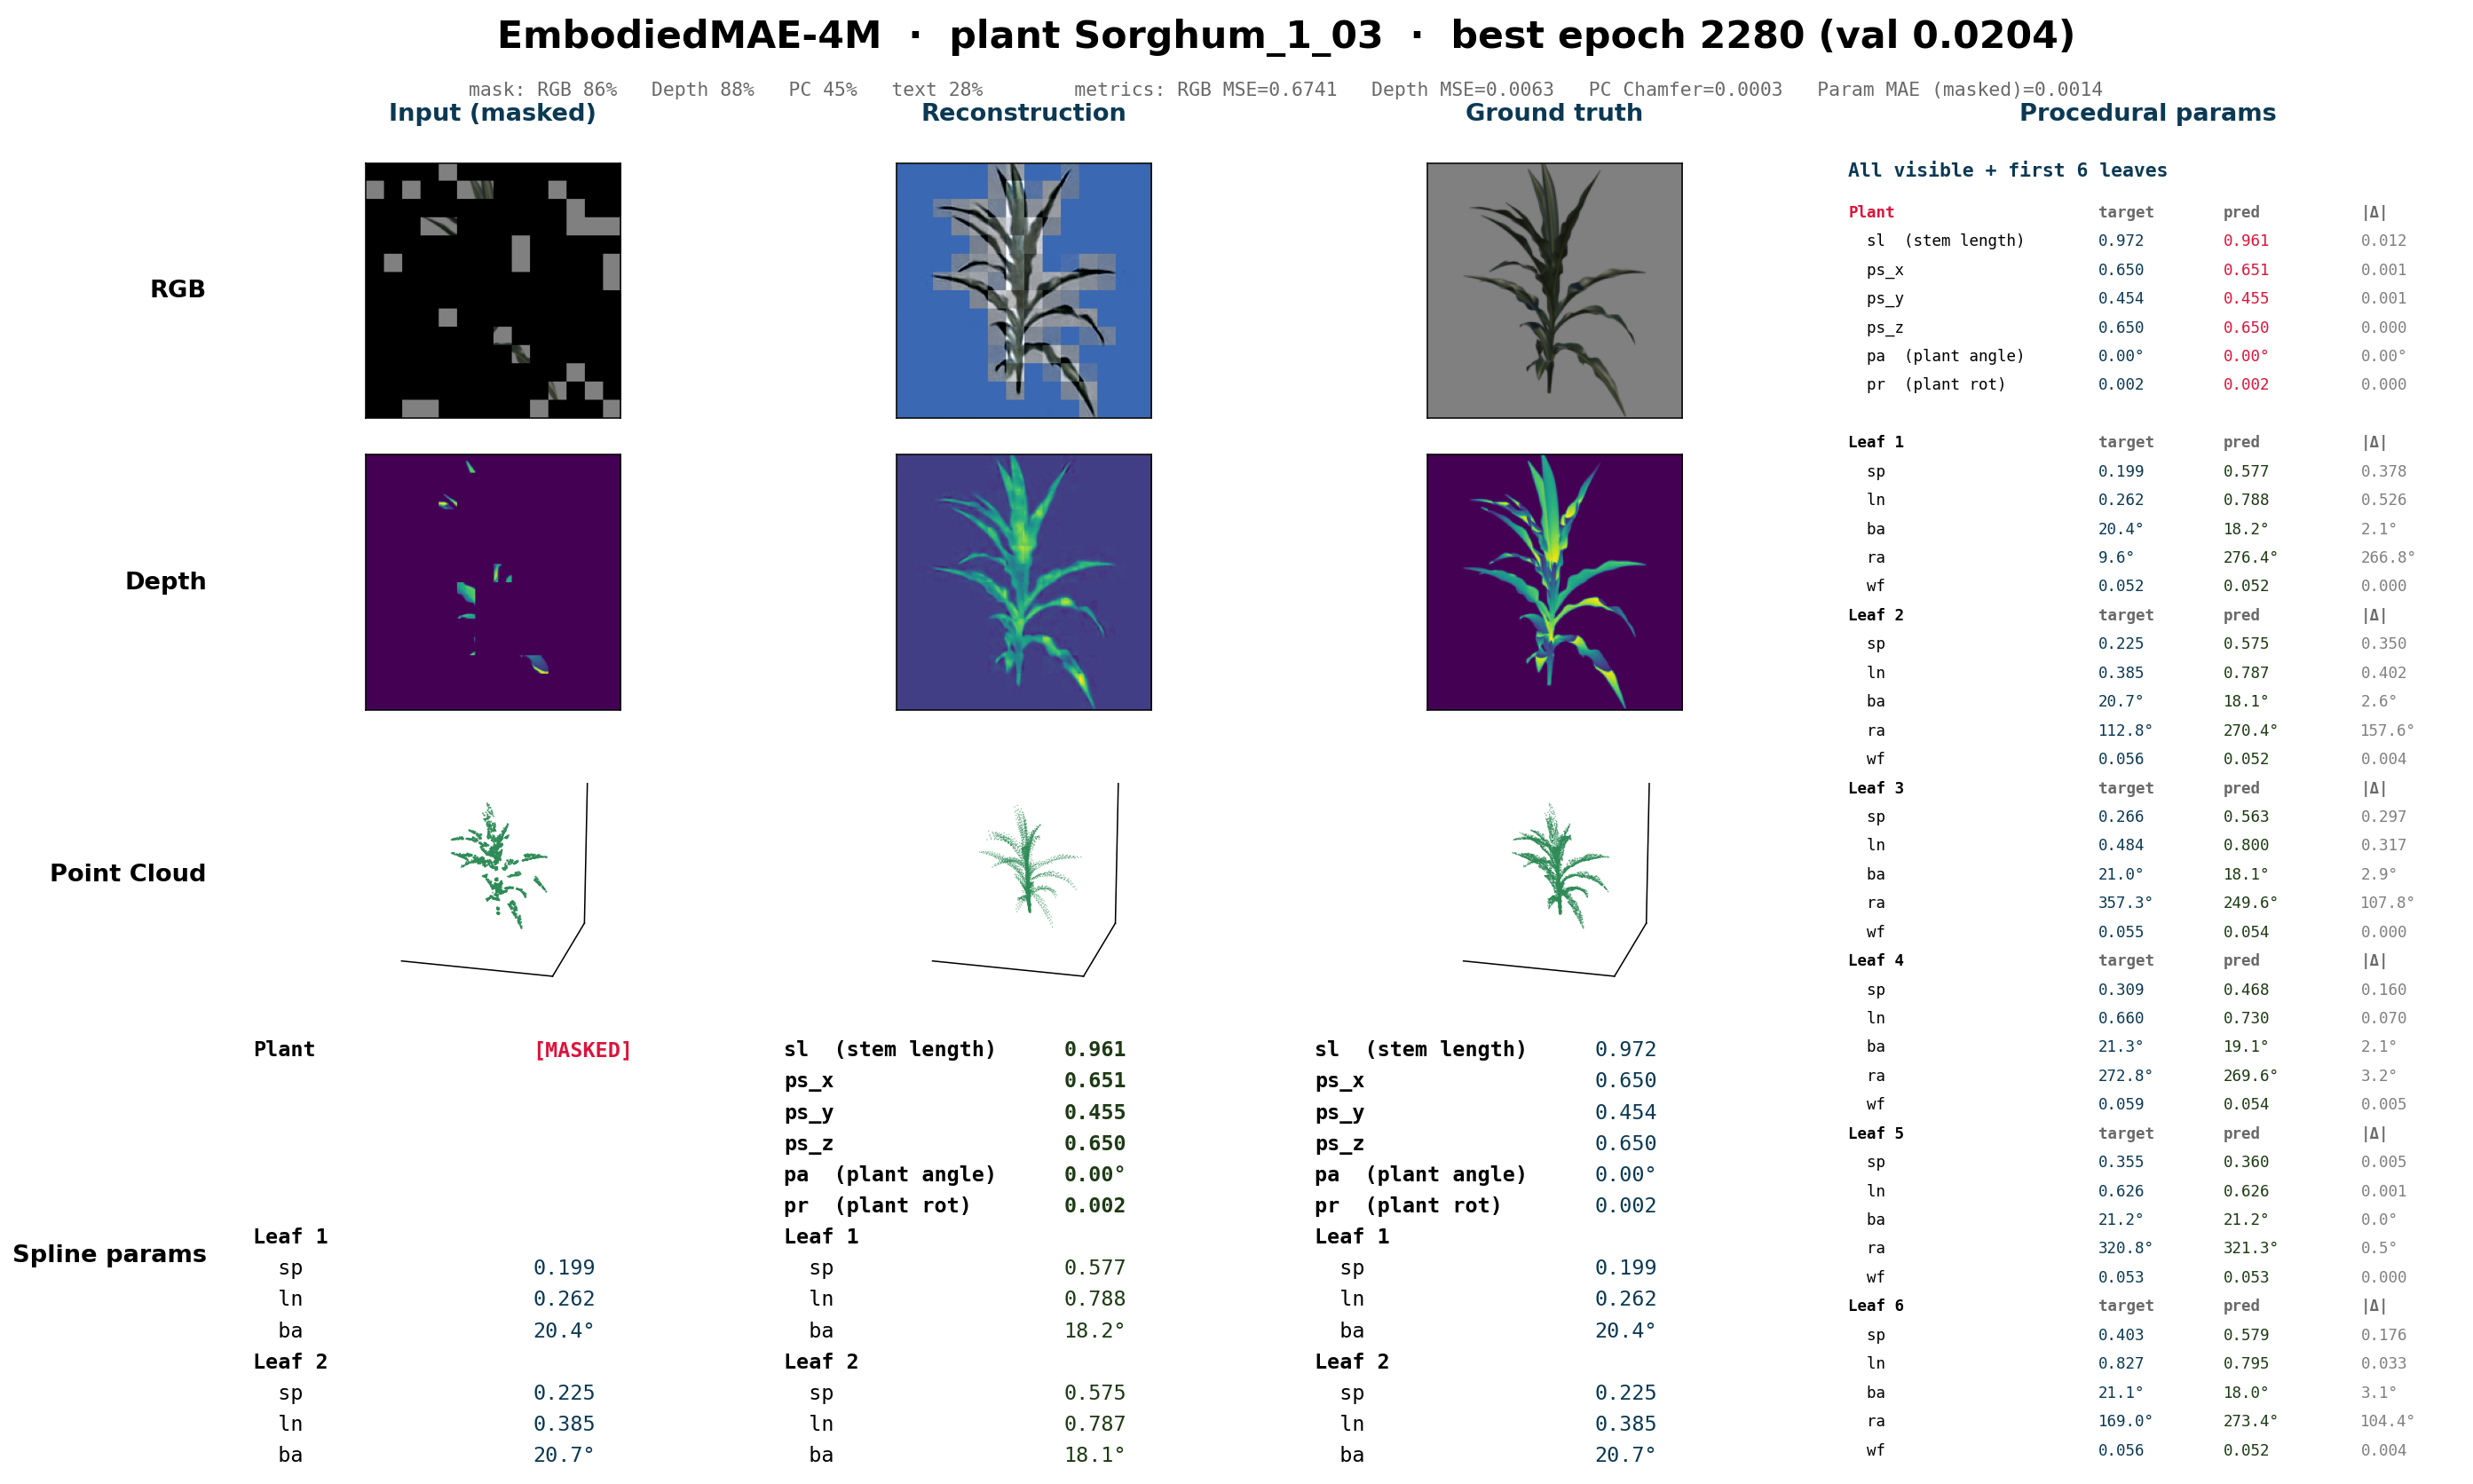
\includegraphics[width=\linewidth]{per_plant/Sorghum_1_03.png}
\caption{Plant Sorghum\_1\_03 -- epoch 2400 reconstruction.}
\label{fig:plant:Sorghum_1_03}
\end{figure}
\clearpage

\begin{figure}[H]
\centering
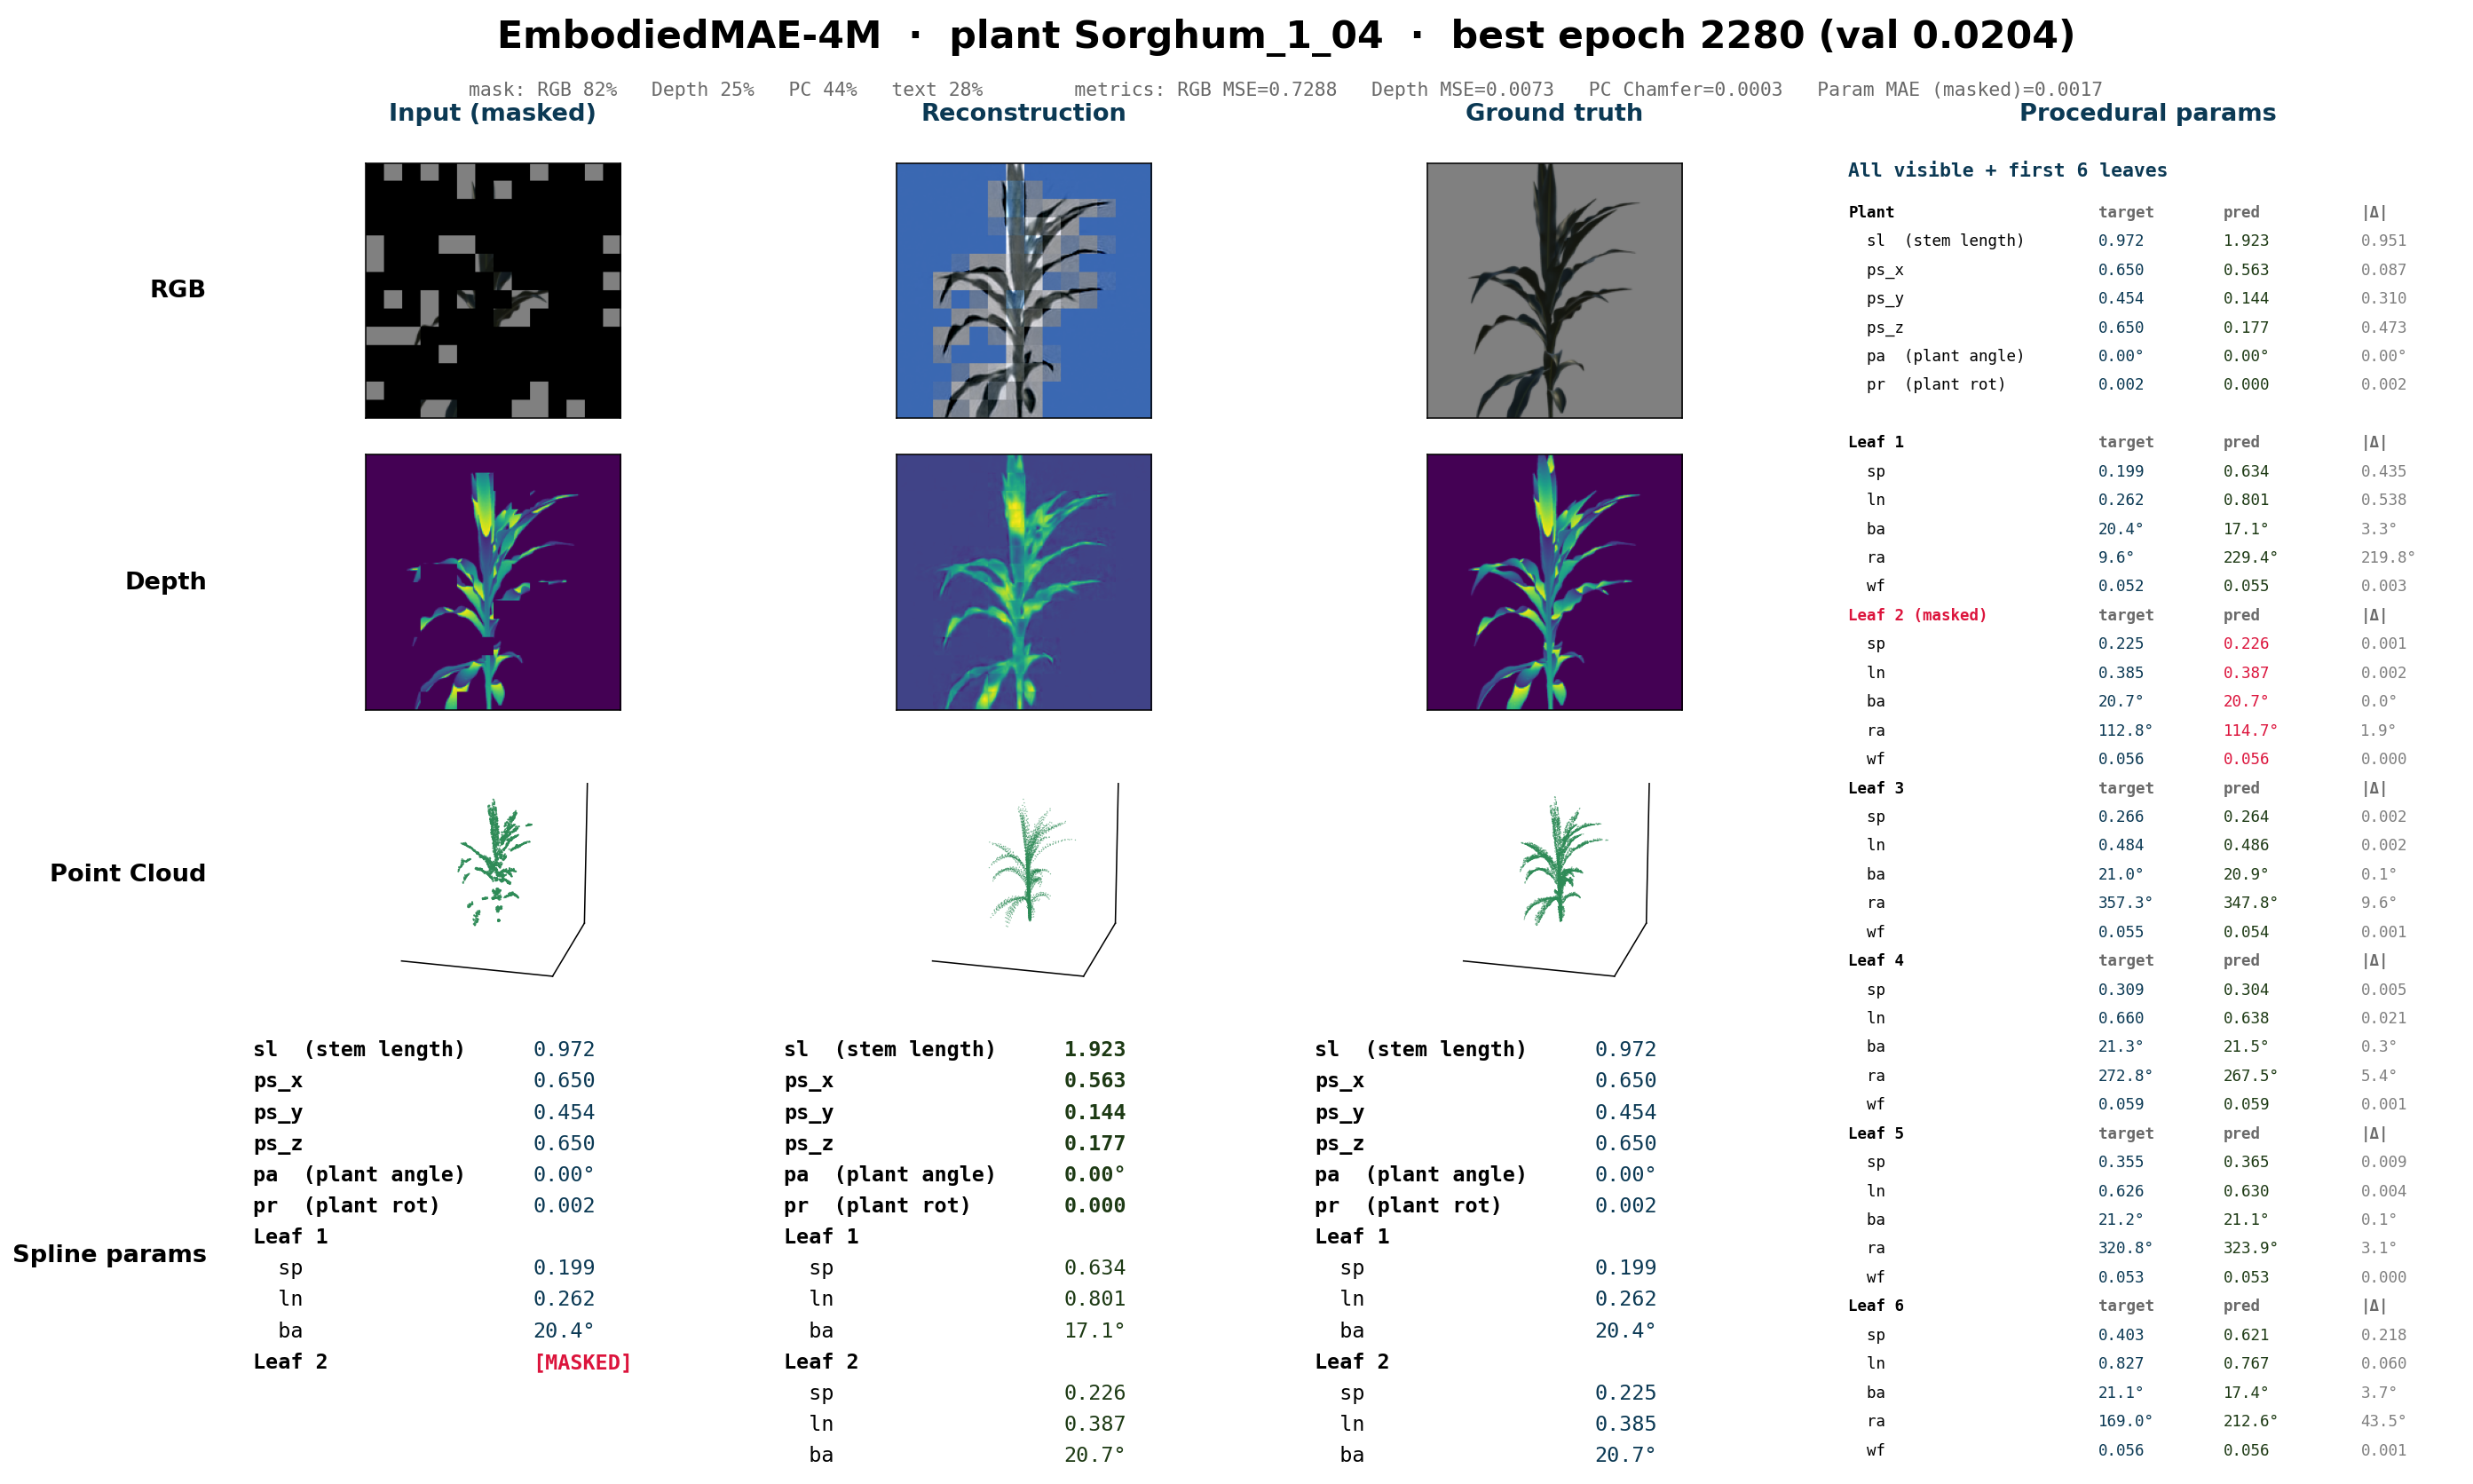
\includegraphics[width=\linewidth]{per_plant/Sorghum_1_04.png}
\caption{Plant Sorghum\_1\_04 -- epoch 2400 reconstruction.}
\label{fig:plant:Sorghum_1_04}
\end{figure}
\clearpage

\end{document}
